% Options for packages loaded elsewhere
\PassOptionsToPackage{unicode}{hyperref}
\PassOptionsToPackage{hyphens}{url}
\PassOptionsToPackage{dvipsnames,svgnames,x11names}{xcolor}
%
\documentclass[
]{article}
\usepackage{amsmath,amssymb}
\usepackage{iftex}
\ifPDFTeX
  \usepackage[T1]{fontenc}
  \usepackage[utf8]{inputenc}
  \usepackage{textcomp} % provide euro and other symbols
\else % if luatex or xetex
  \usepackage{unicode-math} % this also loads fontspec
  \defaultfontfeatures{Scale=MatchLowercase}
  \defaultfontfeatures[\rmfamily]{Ligatures=TeX,Scale=1}
\fi
\usepackage{lmodern}
\ifPDFTeX\else
  % xetex/luatex font selection
\fi
% Use upquote if available, for straight quotes in verbatim environments
\IfFileExists{upquote.sty}{\usepackage{upquote}}{}
\IfFileExists{microtype.sty}{% use microtype if available
  \usepackage[]{microtype}
  \UseMicrotypeSet[protrusion]{basicmath} % disable protrusion for tt fonts
}{}
\makeatletter
\@ifundefined{KOMAClassName}{% if non-KOMA class
  \IfFileExists{parskip.sty}{%
    \usepackage{parskip}
  }{% else
    \setlength{\parindent}{0pt}
    \setlength{\parskip}{6pt plus 2pt minus 1pt}}
}{% if KOMA class
  \KOMAoptions{parskip=half}}
\makeatother
\usepackage{xcolor}
\usepackage{color}
\usepackage{fancyvrb}
\newcommand{\VerbBar}{|}
\newcommand{\VERB}{\Verb[commandchars=\\\{\}]}
\DefineVerbatimEnvironment{Highlighting}{Verbatim}{commandchars=\\\{\}}
% Add ',fontsize=\small' for more characters per line
\newenvironment{Shaded}{}{}
\newcommand{\AlertTok}[1]{\textcolor[rgb]{1.00,0.00,0.00}{\textbf{#1}}}
\newcommand{\AnnotationTok}[1]{\textcolor[rgb]{0.38,0.63,0.69}{\textbf{\textit{#1}}}}
\newcommand{\AttributeTok}[1]{\textcolor[rgb]{0.49,0.56,0.16}{#1}}
\newcommand{\BaseNTok}[1]{\textcolor[rgb]{0.25,0.63,0.44}{#1}}
\newcommand{\BuiltInTok}[1]{\textcolor[rgb]{0.00,0.50,0.00}{#1}}
\newcommand{\CharTok}[1]{\textcolor[rgb]{0.25,0.44,0.63}{#1}}
\newcommand{\CommentTok}[1]{\textcolor[rgb]{0.38,0.63,0.69}{\textit{#1}}}
\newcommand{\CommentVarTok}[1]{\textcolor[rgb]{0.38,0.63,0.69}{\textbf{\textit{#1}}}}
\newcommand{\ConstantTok}[1]{\textcolor[rgb]{0.53,0.00,0.00}{#1}}
\newcommand{\ControlFlowTok}[1]{\textcolor[rgb]{0.00,0.44,0.13}{\textbf{#1}}}
\newcommand{\DataTypeTok}[1]{\textcolor[rgb]{0.56,0.13,0.00}{#1}}
\newcommand{\DecValTok}[1]{\textcolor[rgb]{0.25,0.63,0.44}{#1}}
\newcommand{\DocumentationTok}[1]{\textcolor[rgb]{0.73,0.13,0.13}{\textit{#1}}}
\newcommand{\ErrorTok}[1]{\textcolor[rgb]{1.00,0.00,0.00}{\textbf{#1}}}
\newcommand{\ExtensionTok}[1]{#1}
\newcommand{\FloatTok}[1]{\textcolor[rgb]{0.25,0.63,0.44}{#1}}
\newcommand{\FunctionTok}[1]{\textcolor[rgb]{0.02,0.16,0.49}{#1}}
\newcommand{\ImportTok}[1]{\textcolor[rgb]{0.00,0.50,0.00}{\textbf{#1}}}
\newcommand{\InformationTok}[1]{\textcolor[rgb]{0.38,0.63,0.69}{\textbf{\textit{#1}}}}
\newcommand{\KeywordTok}[1]{\textcolor[rgb]{0.00,0.44,0.13}{\textbf{#1}}}
\newcommand{\NormalTok}[1]{#1}
\newcommand{\OperatorTok}[1]{\textcolor[rgb]{0.40,0.40,0.40}{#1}}
\newcommand{\OtherTok}[1]{\textcolor[rgb]{0.00,0.44,0.13}{#1}}
\newcommand{\PreprocessorTok}[1]{\textcolor[rgb]{0.74,0.48,0.00}{#1}}
\newcommand{\RegionMarkerTok}[1]{#1}
\newcommand{\SpecialCharTok}[1]{\textcolor[rgb]{0.25,0.44,0.63}{#1}}
\newcommand{\SpecialStringTok}[1]{\textcolor[rgb]{0.73,0.40,0.53}{#1}}
\newcommand{\StringTok}[1]{\textcolor[rgb]{0.25,0.44,0.63}{#1}}
\newcommand{\VariableTok}[1]{\textcolor[rgb]{0.10,0.09,0.49}{#1}}
\newcommand{\VerbatimStringTok}[1]{\textcolor[rgb]{0.25,0.44,0.63}{#1}}
\newcommand{\WarningTok}[1]{\textcolor[rgb]{0.38,0.63,0.69}{\textbf{\textit{#1}}}}
\usepackage{graphicx}
\makeatletter
\def\maxwidth{\ifdim\Gin@nat@width>\linewidth\linewidth\else\Gin@nat@width\fi}
\def\maxheight{\ifdim\Gin@nat@height>\textheight\textheight\else\Gin@nat@height\fi}
\makeatother
% Scale images if necessary, so that they will not overflow the page
% margins by default, and it is still possible to overwrite the defaults
% using explicit options in \includegraphics[width, height, ...]{}
\setkeys{Gin}{width=\maxwidth,height=\maxheight,keepaspectratio}
% Set default figure placement to htbp
\makeatletter
\def\fps@figure{htbp}
\makeatother
\setlength{\emergencystretch}{3em} % prevent overfull lines
\providecommand{\tightlist}{%
  \setlength{\itemsep}{0pt}\setlength{\parskip}{0pt}}
\setcounter{secnumdepth}{-\maxdimen} % remove section numbering
\usepackage{preamble_ai_project}
\usepackage[backend=bibtex,style=numeric]{biblatex}
\bibliography{references}
\usepackage{algorithm}
\usepackage{algpseudocode}
\newcommand{\w}{\mathbf{w}}
\newcommand{\x}{\mathbf{x}}
\ifLuaTeX
  \usepackage{selnolig}  % disable illegal ligatures
\fi
\usepackage{bookmark}
\IfFileExists{xurl.sty}{\usepackage{xurl}}{} % add URL line breaks if available
\urlstyle{same}
\hypersetup{
  colorlinks=true,
  linkcolor={Blue},
  filecolor={Maroon},
  citecolor={Blue},
  urlcolor={Blue},
  pdfcreator={LaTeX via pandoc}}

\author{}
\date{}

\begin{document}

\intro{}

\section{1 -- Introduction \& Rappels
théoriques}\label{introduction-rappels-thuxe9oriques}

Dans ce document, nous approfondirons les techniques de ``Régression
logistique'' et ``Naive Bayes'' comme outils d'apprentissage supervisés.

Dans le cadre de l'intelligence artificielle et de l'apprentissage
supervisé, la compréhension et la classification précise des données
revêtent une importance capitale. Parmi les diverses méthodologies
existantes, la ``Régression Logistique'' et ``Naive Bayes'' se
distinguent par leur efficacité et leur applicabilité dans de nombreux
contextes. Ce document se propose d'étudier ces deux techniques, en
mettant l'accent sur leur mise en œuvre pratique et leur efficacité
comparative dans divers scénarios.

\subsection{1.1 -- Régression
Logistique}\label{ruxe9gression-logistique}

En statistiques, la régression logistique s'inscrit dans le cadre des
modèles de régression pour les variables binaires. Bien qu'elle soit
quasiment exclusivement utilisée en tant que méthode de
classification.\\
En effet, c'est l'ajout d'un seuil à la probabilité continue donnée par
le modèle de régression qui nous permet de l'utiliser pour la
classification.

Ce type de modèle vise à expliquer de manière optimale une variable
binaire, qui représente la présence ou l'absence d'une caractéristique
spécifique, à l'aide d'un ensemble conséquent de données réelles et d'un
modèle mathématique.

Autrement dit, il s'agit de relier une variable aléatoire de Bernoulli,
généralement notée \(y\), aussi appelé ``label'' à un vecteur constitué
de plusieurs variables aléatoires, \((x_1, \ldots, x_K)\), aussi appelés
``features''. \cite{RegressionLogistique2023}.

La régression logistique s'appuie sur un classifeur linéaire
\cite{ClassifieurLineaire2022} i.e.~un classifieur dont la sortie (pour
un vecteur de feature \(x \in \R^n\)) est donnée par:

\[
g(x) = f(\scalproduct{w}{x} + b)
\] où \(w \in \R^n\) est le vecteur de poids, \(b \in \R\) le biais et
\(\scalproduct{.}{.}\) le produit scalaire usuel. \(f\) est une fonction
dite de seuillage qui va séparer nos résultats. Un choix commun pour
\(f\) est la sigmoide ou la fonction signe
\cite{ClassifieurLineaire2022}.

Par exemple, dans le cas de la regression logistique binaire, on suppose
le modèle suivant:

\[
y_i \sim Bernoulli(p_i),\quad p_i = \sigma(\scalproduct{\mathbf{w}}{\mathbf{x}_i} + b),\quad \sigma(z) = \frac{1}{1 + e^{-z}}
\] où \(\mathbf{x}_i \in \R^K\) représente un vecteur (ligne) de \(K\)
valeurs pour les \(K\) features (aussi appelé un \emph{sample}), et
\(y_i\) la variable aléatoire qui représente le label qui leur est
associé.

Cependant, dans notre dataset (voir
\href{#choix-du-dataset-outils-utilisuxe9s}{section 2.0}) nous avons 3
classes (3 espèces d'iris), \(y\) ne suit donc, évidemment, plus une loi
de Bernoulli.

La sigmoide étant continue, nous avons testé 2 méthodes de prédiction:

\begin{itemize}
\tightlist
\item
  La première consistait simplement à modifier la manière dont nous
  appliquions le seuillage sur la fonction sigmoide, pour distinguer 3
  cas au lieu de 2. i.e.~Au lieu de séparer le domaine en 2
  (\(\sigma(z) \leq 0.5,\ \sigma(z) > 0.5\)), nous l'avons séparé en
  \(N\) (ici \(N = 3\)). On a donc que
  \(y_i = k \Leftrightarrow \frac{k}{N} \leq \sigma(z) < \frac{k + 1}{N}\),
  ce qui a donné des résultats assez satisfaisants comme nous le verrons
  en \href{#ruxe9gression-logistique-1}{section 2.2}.
\item
  La deuxième consistait évidement en l'application non pas de la
  régression logistique binaire, mais de la régression logistique
  multinomiale, fonctionnant avec plusieurs labels. Le principe de la
  régression logistique multinomiale est simplement de faire plusieurs
  régressions logistiques binaires. On possède donc un vecteur de poids
  et un biais par label, et on calcule à chaque fois la probabilité que
  l'élément appartienne à une certaine classe. La prédiction retournera
  la classe pour laquelle la probabilité que l'élément appartienne à la
  classe est la plus élevée.
\end{itemize}

\subsection{1.2 -- Naive Bayes}\label{naive-bayes}

``Naive Bayes'' se présente comme une méthode de classification
probabiliste basée sur le
\href{https://en.wikipedia.org/wiki/Bayes\%27_theorem}{théorème de
Bayes}, caractérisée par l'adoption d'une hypothèse d'indépendance forte
entre les features (attributs), qualifiée de ``naïve''.\\
Plus simplement, le classifieur est considéré comme ``naïf'' car il part
du principe que chaque feature (attribut) est indépendante des autres et
a un poid égal quant à la probabilité qu'un point appartienne à une
classe.

Ce modèle est dit génératif contrairement à la régression logistique,
étant considéré comme ``méthode discriminante''
\cite{ClassifieurLineaire2022}, et consiste à modéliser les probabilités
conditionnelles \(P(\mathbf{x}| classe)\) pour chaque classe \(y\) et
smaple \(\mathbf{x}\) afin de trouver celle qui maximise cette
probabilité.

En d'autres termes, le problème revient à trouver, pour des attributs
\(x_1, \ldots, x_k\), la classe \(\tilde{y}\) telle que:

\[
\tilde{y} = \text{arg}\max_{y \in \mathcal{Y}} \left[\  P(y) \prod_{k = 1}^K{P(x_k | Y)}\  \right]
\]

\newpage

\section{2 -- Méthodologie}\label{muxe9thodologie}

\subsection{2.0 -- Choix du dataset \& outils
utilisés}\label{choix-du-dataset-outils-utilisuxe9s}

Pour la suite de ce projet les outils suivants ont été utilisés dans
chaque parties:

\begin{itemize}
\tightlist
\item
  \href{https://www.python.org/}{python}
\item
  \href{https://python-poetry.org/}{poetry}
\item
  \href{https://www.gnu.org/software/make/}{Make}
\item
  \href{https://numpy.org/}{numpy}
\item
  \href{https://pandas.pydata.org/}{pandas}
\item
  \href{https://scikit-learn.org/stable/}{sklearn}
\item
  \href{https://matplotlib.org/}{matplotlib}
\item
  \href{https://github.com/uci-ml-repo/ucimlrepo}{ucmilrepo}
\item
  \href{https://docs.pytest.org/en/stable/}{pytest}
\end{itemize}

Le package \texttt{ucmilrepo} a été utilisé pour charger les données de
notre dataset depuis la base de donnée du
\href{https://archive.ics.uci.edu/ml/index}{UC Irvine Machine Learning
Repository}.

Le dataset que nous avons choisi est le fameux dataset ``Iris''
\cite{r.a.fisherIris1936}, un des plus anciens et connus dataset de
classification. Il contient 150 observations de 3 espèces différentes
d'iris (Iris setosa, Iris virginica et Iris versicolor) avec \(K = 4\)
features (longueur et largeur des sépales et pétales).

Voici un aperçu des points-clés du dataset:

\begin{figure}
\centering
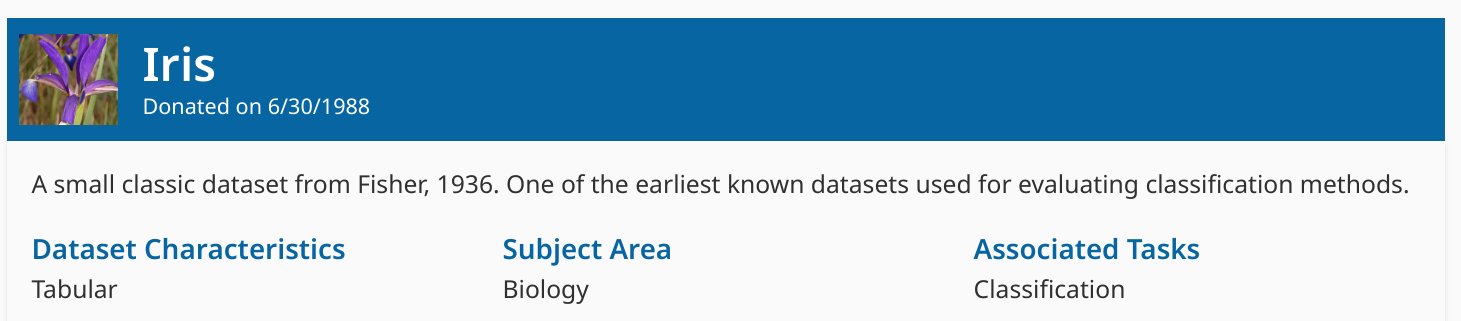
\includegraphics[width=0.8\textwidth,height=\textheight]{../res/iris_img.png}
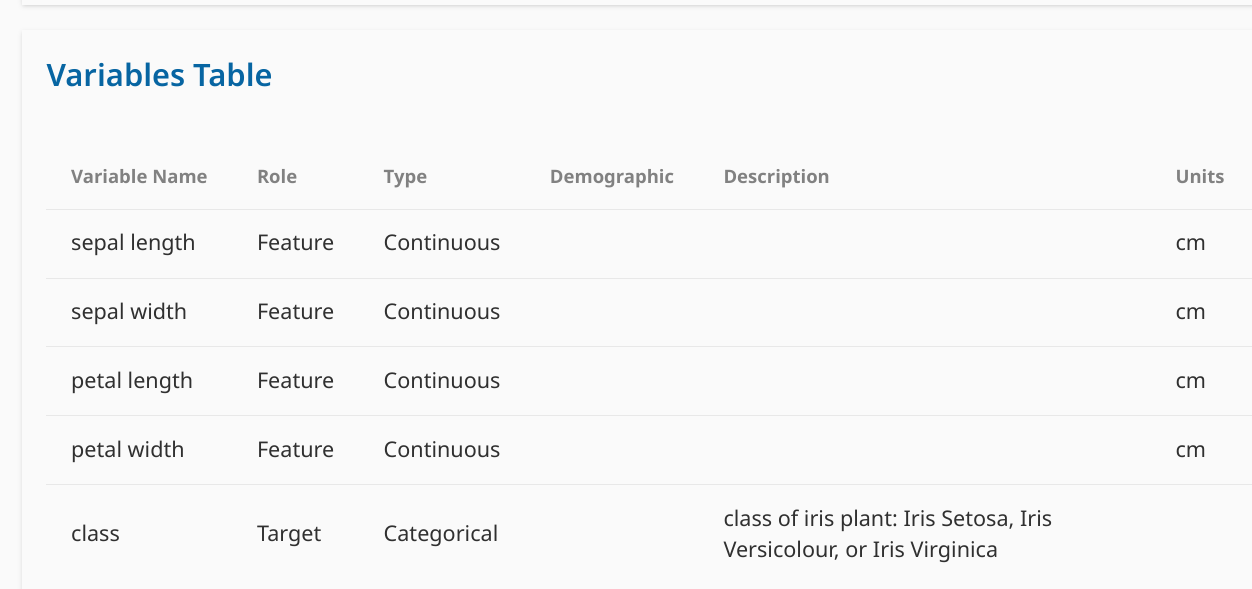
\includegraphics[width=0.8\textwidth,height=\textheight]{../res/iris_table.png}
\caption{Iris descriptive table}
\end{figure}

Le label que nous allons prédire sera donc \emph{class}, i.e.~l'espèce
de l'iris.

\newpage

\subsection{2.1 -- Gradient Descent}\label{gradient-descent}

Dans cette section, une implémentation de la ``descente en gradient'' a
été réalisée. La fonction a la signature suivante

\begin{lstlisting}
  def gradient_descent(df, params: NDArray, alpha: float, num_iters: int) -> NDArray:  
\end{lstlisting}

Elle calcule de manière itérative le(s) paramètre(s) \code{params} qui
minimisent la fonction dont \texttt{df} est le gradient avec un ``taux
de convergence'' \code{alpha}.

La fonction a été testé avec la fonction \code{scipy.optimize.fmin}
\cite{ScipyOptimizeFmin} de la librairie \texttt{scipy} sur la fonction
suivante: \[
f(x) = x * \cos(\pi  (x + 1))
\]

avec différents \(x_0 \in \{-\pi, 0, \pi\}\) (valeur initiale de
\code{params}, i.e.~\texttt{NDArray} avec D=0).

Les minimas locaux trouvés par les deux fonctions sont les suivants:

\begin{figure}
\centering
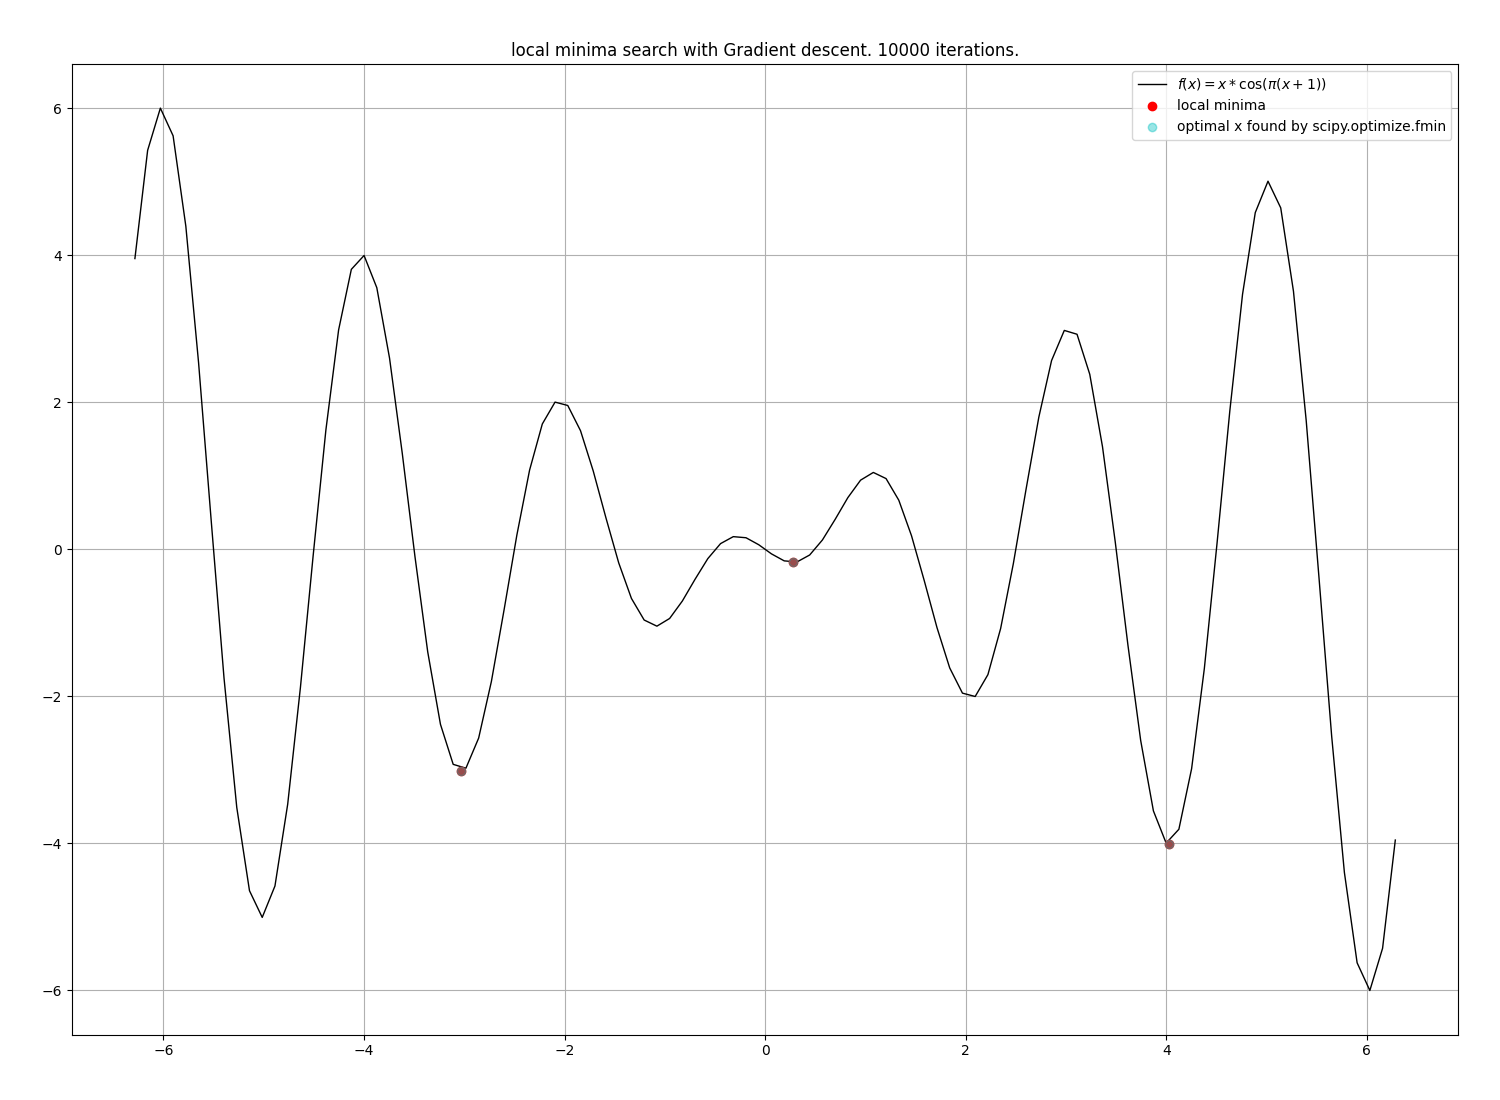
\includegraphics[width=1\textwidth,height=\textheight]{../res/3.1_gradient_descent_minima.png}
\caption{minimas locaux\_gradient descent}
\end{figure}

Ce résultat illustre bien 2 choses: la première est que l'implémentation
de la descente en gradient fonctionne correctement puisque chaque points
trouvé par notre fonction est confondu avec celui trouvé par la fonction
de scipy (c'est ce qui donne cette teinte ``grise''). La deuxième est
que la ``qualité'' du minima local (i.e.~la distance avec le minima
globale) dépend fortement de la valeur initiale et ce pour les deux
fonctions.

\newpage{}

\subsection{2.2 -- Régression
Logistique}\label{ruxe9gression-logistique-1}

\subsubsection{2.2.1 -- Fonction de coût pour la régression logistique
binaire}\label{fonction-de-couxfbt-pour-la-ruxe9gression-logistique-binaire}

\paragraph{2.2.1.1 -- Fonction de coût}\label{fonction-de-couxfbt}

Reprennons le modèle décrit dans la section 1.1. Nous avons donc:
\[y_i \sim Bernoulli(p_i), p_i = \sigma(w^T x_i + b), \sigma(z) = \frac{1}{1+e^{-z}}\]

Notre but est de calculer \(p(y_i | x_i)\), puis de seuiller le résultat
obtenu afin de prédire si l'élément possédant les caractéristiques
\(x_i\) appartient ou pas à la classe \(y_i\). On cherche donc à trouver
les paramètres de poids \(w\) et de biais \(b\) optimaux permettant la
meilleure prédiction possible. On peut trouver la notation
\(p(y_i|x_i;w, b)\) indiquant que nous ne connaissons pas encore le
vecteur poids \(w\) et le biais \(b\).

La densité de probabilité de cette fonction peut donc s'exprimer comme

\[p(y_i|x_i; w, b) = p_i^{y_i}(1 - p_i)^{1 - y_i}\]

Notre but est donc de maximiser cette fonction. Cependant, nous
préférons une fonction à minimiser plutôt qu'à maximiser, car la
descente en gradient permet de trouver un minimum et non pas un
maximum\ldots{}

Une solution habituelle est donc d'inverser la fonction, transformant
ainsi le problème de maximisation en problème de minimisation, et de
prendre le logarithme de l'inverse de cette fonction afin d'éviter des
valeurs extrêmes lors de notre minimisation. L'application de la
fonction logarithme sur l'inverse de la fonction est correcte car la
fonction logarithme est strictement croissante, donc elle n'aura pas
d'impact sur la convexité de la fonction. Cette solution est communément
appelée \texttt{Negative\ Logarithm\ Likelihood}.

Donc on cherchera à minimiser la fonction:
\[log\left(\frac{1}{p(y_i|x_i;w,b)}\right) = log(1) - log(p(y_i|x_i;w,b)) = -log(p(y_i|x_i; w, b)\]
Pour \(n\) données, cette fonction peut s'écrire:
\[-\sum_i^n log(p(y_i|x_i;w,b))\]

\paragraph{2.2.1.2 -- Dérivée de la fonction de
coût}\label{duxe9rivuxe9e-de-la-fonction-de-couxfbt}

Comme nous voulons utiliser la descente en gradient, nous devons trouver
la dérivée de la fonction à minimiser, donc de notre fonction de coût.

Tout d'abord, remarquons que nous pouvons écrire:
\[log(p(y_i|x_i; w, b))\] \[= log(p_i^{y_i}(1 - p_i)^{1 - y_i})\]
\[= log(p_i^{y_i}) + log((1 - p_i)^{1 - y_i})\]
\[= y_i log(p_i) + (1 - y_i)log(1 - p_i)\]

De plus, voici ce que nous donne la dérivée de la fonction sigmoide:
\[\frac{d\sigma(z)}{dz}\] \[= ((1 + e^{-z})^{-1})'\]
\[= -1 \times - e ^{-z} \times (1 + e^{-z})^{-2}\]
\[=\frac{e^{-z}}{(1 + e^{-z})^2}\]
\[=\frac{1}{1 + e^{-z}}\frac{e^{-z}}{1 + e^{-z}}\]
\[= \sigma (z) \frac{e^{-z}}{1 + e^{-z}}\]
\[= \sigma (z) \frac{1 + e^{-z} - 1}{1 + e^{-z}}\]
\[= \sigma (z) (\frac{1 + e^{-z}}{1 + e^{-z}} - \frac{1}{1 + e^{-z}})\]
\[= \sigma (z) (1 - \frac{1}{1 + e^{-z}})\]
\[= \sigma (z) (1 - \sigma (z))\]

Donc nous pouvons facilement calculer la dérivée par rapport au poid
\(w\) et par rapport au biais de notre fonction de coût.

Voici ce que nous donne la dérivée partielle par rapport au poids
\(\frac{\partial}{\partial w_j}\):

\[\frac{\partial}{\partial w_j}\left(-log(p(y_i|x_i;w,b))\right)\]

\[=-\frac{\partial}{\partial w_j} (y_i log(p_i) - (1 - y_i)log(1 - p_i))\]
\[=-y_i \frac{\partial}{\partial w_j}log(p_i) - (1 - y_i)\frac{\partial}{\partial w_j}log(1 - p_i)\]
\[=-y_i \frac{\partial}{\partial w_j}log(\sigma (z)) - (1 - y_i)\frac{\partial}{\partial w_j}log(1 - \sigma (z)),\ z = w^T x_i + b\]
\[=-y_i \frac{1}{\sigma (z)}\frac{\partial}{\partial w_j}\sigma (z) - (1 - y_i)\frac{1}{1 - \sigma (z)}\frac{\partial}{\partial w_j}(1 - \sigma (z))\]

Or on a:
\[\frac{\partial}{\partial w_j} z = \frac{\partial}{\partial w_j}(w^T x_i + b) \Leftrightarrow \frac{dz}{\partial w_j} = x_{ij} \Leftrightarrow \frac{\partial}{\partial w_j} = \frac{d}{dz}x_{ij}\]

Donc:
\[-y_i \frac{1}{\sigma (z)}\frac{\partial}{\partial w_j}\sigma (z) - (1 - y_i)\frac{1}{1 - \sigma (z)}\frac{\partial}{\partial w_j}(1 - \sigma (z))\]

\[=-y_i \frac{1}{\sigma (z)}\frac{d}{dz}\sigma (z)x_{ij} - (1 - y_i)\frac{1}{1 - \sigma (z)}\left(-\frac{d}{dz} \sigma (z)x_{ij}\right)\]
\[=-y_i \frac{1}{\sigma (z)}\sigma (z) (1 - \sigma (z)) x_{ij} - (1 - y_i)\frac{1}{1 - \sigma (z)}(- \sigma (z))(1 - \sigma(z))x_{ij}\]
\[=-y_i (1 - \sigma (z)) x_{ij} + (1 - y_i)\sigma (z)x_{ij}\]
\[=-y_i x_{ij} + y_i \sigma (z) x_{ij} + (1 - y_i)\sigma (z)x_{ij}\]
\[=-y_i x_{ij} + (y_i + 1 - y_i)\sigma (z)x_{ij}\]
\[=(\sigma(z) - y_i)x_{ij}\]

Voici ce que nous donne la dérivée partielle par rapport au biais
\(\frac{\partial}{\partial b}\):

\[\frac{\partial}{\partial b}\left(-log(p(yi|xi;w,b))\right)\]

\[=-\frac{\partial}{\partial b}(y_i log(p_i) + (1 - y_i)log(1 - p_i))\]
\[=-y_i \frac{\partial}{\partial b}log(p_i) - (1 - y_i)\frac{\partial}{\partial b}log(1 - p_i)\]
\[=-y_i \frac{1}{\sigma (z)}\frac{\partial}{\partial b} \sigma(z) - (1 - y_i) \frac{1}{1 - \sigma (z)} \frac{\partial}{\partial b}(1 - \sigma (z)),\ z = w^T x_i + b\]

On a:

\[\frac{\partial}{\partial b} z = \frac{\partial}{\partial b}(w^T x_i + b) \Leftrightarrow \frac{dz}{db} = 1 \Leftrightarrow \frac{\partial}{\partial b} = \frac{d}{dz}\]

Donc:
\[-y_i \frac{1}{\sigma (z)}\frac{\partial}{\partial b} \sigma(z) - (1 - y_i) \frac{1}{1 - \sigma (z)} \frac{\partial}{\partial b}(1 - \sigma (z))\]
\[=-y_i \frac{1}{\sigma (z)}\frac{d}{dz} \sigma(z) - (1 - y_i) \frac{1}{1 - \sigma (z)} \frac{d}{dz}(1 - \sigma (z))\]
\[=-y_i \frac{1}{\sigma (z)}\frac{d}{dz} \sigma(z) + (1 - y_i) \frac{1}{1 - \sigma (z)} \frac{d}{dz}\sigma (z)\]
\[=-y_i \frac{1}{\sigma (z)}\sigma(z) (1 - \sigma (z)) + (1 - y_i) \frac{1}{1 - \sigma (z)} \sigma (z)(1 - \sigma (z))\]
\[=-y_i (1 - \sigma (z)) + (1 - y_i)\sigma (z)\]
\[=-y_i + y_i \sigma (z) + (1 - y_i)\sigma (z)\]
\[=-y_i + (y_i + 1 - y_i)\sigma (z)\] \[=\sigma (z) - y_i\]

Donc pour \(n\) données, la dérivée de la fonction de coût par rapport
au poids et au bias nous donne:

\[\frac{\partial}{\partial w_j}\left( - \sum_i^n log(p(y_i|x_i;w,b))\right) = \sum_i^n(\sigma(z) - y_i)x_{ij}\]

et:

\[\frac{\partial}{\partial b}\left(- \sum_i^n log(p(yi|xi;w,b))\right) = \sum_i^n (\sigma (z) - y_i)\]

\subsubsection{2.2.2 -- Fonction de coût pour la régression logistique
multinomiale}\label{fonction-de-couxfbt-pour-la-ruxe9gression-logistique-multinomiale}

Afin d'entraîner les paramètres de la régression logistique, il faut
pouvoir comparer les résultats obtenus par la régression avec les
résultats attendus.

On souhaite définir une fonction à minimiser permettant de trouver les
paramètres optimaux de la régression logistique.

Notre classification se base sur la fonction sigmoïde
\(\sigma(z) = \frac{1}{1 + e^{-z}}\).

Comme la fonction exponnentielle est toujours positive, on a bien que
\(\sigma(z) \in [0, 1]\).

La fonction sigmoïde nous donne la probabilité que l'élément donné
appartienne à un label.

Autrement dit, la fonction sigmoïde est la fonction de répartition de la
régression logistique.

Soit \(Y \in \{0, 1\}\) les différents labels que peut prendre l'élément
que l'on considère et soit \(X\) l'ensemble des caractéristiques connues
de l'élément, dont on cherche à déterminer dans quelle classe le mettre,
donc quel label on doit lui attribuer. Soit \(\theta\) le vecteur des
poids des covariables, indiquant à quel point les covariables
influencent sur la décision du label. On a donc:

\[P(Y = 1 | X) = \frac{1}{1 + e^{-(X_1 * w_1 + X_2*w_2 + \dots + b)}}\]
et \[P(Y = 0 | X) = 1 - \frac{1}{1 + e^{-(X_1 * w_1 + \dots + b)}}\]

Pour plus de simplicité, on va considérer que le biais est compris dans
les poids: au lieu d'écrire \(z = wX + b\), on écrit
\(z = \hat{X}\theta\) avec
\(\hat{X} = \begin{bmatrix} X & 1 \end{bmatrix}\) modifié ou on a ajouté
une colonne avec que des \(1\) à la fin de la matrice \(X\) et
\(\theta = \begin{bmatrix} w & b \end{bmatrix}\) afin d'avoir une bonne
cohérence avec le rapport et le code. (On a trouvé cela plus facile
d'avoir pour chaque labels les poids et bias sur une ligne, donc d'avoir
\(\theta_1\) pour le label \(1\) etc\ldots) Ainsi, on a:
\(\hat{X} \theta^T = X_1 * w_1 + X_2 * w_2 + \dots + b\)

Pour la suite, on va noter \(X = \hat{X}\)

Notre régression logistique binaire peut donc s'écrire comme:
\[P(Y = 1 | X) = \frac{1}{1 + e^{X \theta^T}} = \sigma(X \theta^T)\] et
\[P(Y = 0 | X) = 1 - \sigma(X \theta^T)\]

\paragraph{2.2.2.1 -- Généralisation de la régression logistique
binaire}\label{guxe9nuxe9ralisation-de-la-ruxe9gression-logistique-binaire}

On désire donc trouver une nouvelle distribution \(\phi(z)\) tel que:
\[\phi(z) \in [0, 1]\ \forall z\] est une généralisation de la fonction
\(\sigma(z)\)

On veut donc que pour une régression logistique binaire, on ait
\(\sigma(z) = \phi(z)\).

On peut remarquer que:

\[P(Y = 1 | X)\] \[=\frac{1}{1 + e^{-X \theta^T}}\]
\[=\frac{1}{1 + e^{-X \theta^T}} * \frac{e^{X \theta^T}}{e^{X \theta^T}}\]
\[=\frac{e^{X \theta^T}}{e^{X \theta^T} + e^{X \theta^T - X \theta^T}}\]
\[=\frac{e^{X \theta^T}}{e^{X \theta^T} + e^0}\]
\[=\frac{e^{X \theta^T}}{e^{X \theta^T} + 1}\]

On peut considérer que nous avons un vecteur de poids pour chaque label.

Ainsi, on a \(\theta_0 = \begin{bmatrix} w_0 & b_0 \end{bmatrix}\) pour
le label 0 et \(\theta_1 = \begin{bmatrix} w_0 & b_0 \end{bmatrix}\)
pour le label 1.

Comme on a besoin seulement d'un vecteur de poids pour déterminer le
label de nouveaux éléments avec leurs caractéristiques, on peut
considérer que
\(\theta_0 = \begin{bmatrix} 0 & \dots & 0 \end{bmatrix}\).

Ainsi, la formule précédente nous donne:

\[P(Y = 1 | X)\] \[=\frac{e^{X \theta_1^T}}{e^{X \theta_1^T} + 1}\]
\[=\frac{e^{X \theta_1^T}}{e^{X \theta_1^T} + e^0}\]
\[=\frac{e^{X \theta_1^T}}{e^{X \theta_1^T} + e^{0 * X}}\]
\[=\frac{e^{X \theta_1^T}}{e^{X \theta_1^T} + e^{X \theta_0^T}}\]
\[=\frac{e^{X \theta_1^T}}{\sum_{i = 0}^1 e^{X \theta_i^T}}\]

On peut donc généraliser cette formule pour \(K\) labels.

Cela nous donne:

\[P(Y = k| X )=\frac{e^{X \theta_k^T}}{\sum_{i = 0}^K e^{X \theta_i^T}}\]

Comme la fonction exponentielle est toujours positive, on a bien que:
\[0 \leq e^{X \theta_k^T} \leq e^{X \theta_k^T} + \sum_{i \neq k}^K e^{X \theta_i^T}\]
\[\Leftrightarrow 0 \leq e^{X \theta_k^T} \leq \sum_{i}^K e^{X \theta_i^T}\]
\[\Leftrightarrow 0 \leq \frac{e^{X \theta_k^T}}{\sum_{i}^K e^{X \theta_i^T}} \leq 1\]
\[\Leftrightarrow 0 \leq \phi(z) \leq 1\]

De plus, on a que: \[\sum_k^K P(Y = k | X)\]
\[=\sum_k^K \frac{e^{X \theta_k^T}}{\sum_i^K e^{X \theta_i^T}}\]
\[=\frac{\sum_k^Ke^{X \theta_k^T}}{\sum_i^K e^{X \theta_i^T}}\]
\[=\frac{\sum_i^Ke^{X \theta_i^T}}{\sum_i^K e^{X \theta_i^T}}\] \[=1\]

Donc la fonction \(\phi(z)\) est bien une fonction de distribution de
probabilité qui généralise la fonction sigmoïde pour des problèmes à
plusieurs labels.

Cette fonction est courramment appelée fonction \texttt{softmax}.

\paragraph{2.2.2.2 -- Fonction de coût}\label{fonction-de-couxfbt-1}

Notre objectif est donc de trouver une fonction de coût pour pouvoir
entraîner les paramètres de la régression multinomiale. On cherche à
maximiser la vraisemblance des données. Donc pour un label \(Y\) donné,
on veut maximiser: \[\sum_k^K f(Y, k) P(Y = k | X)\] avec \(f(Y, k)\) la
fonction qui vaut \(1\) si \(Y = k\) et \(0\) sinon.

Comme on a plusieurs couples de données \((X_i, Y_i)\), on peut écrire
la fonction précédente comme:

\[\sum_i^n\sum_k^K f(Y_i, k) P(Y_i = k | X_i)\]

En maximisant cette fonction, on fait en sorte que le paramètre
\(\theta_k\) permette d'obtenir la prédiction que le label soit égal à
\(k\) avec la somme des probabilités où \(Y_i = k\) est la plus grande
possible.

Afin de pouvoir utiliser un algorithme comme la descente en gradient, il
faut non pas maximiser une fonction, mais minimiser une fonction.

Tout d'abord, comme on travaille avec des exponentielles, on a intérêt à
prendre un logarithme pour éviter d'avoir à travailler avec de trop
grandes valeurs. Cette modification n'aura pas d'impact sur la convexité
car la fonction logarithme est une fonction strictement croissante.

Enfin, comme on cherche une fonction à minimiser et non pas à maximiser
pour pouvoir utiliser la descente en gradient, on va prendre l'inverse
de la fonction.

Cela s'appelle courrament le \texttt{negative\ logarithm\ likelihood}.

Cela nous donne une fonction de coût comme suit:

\[\sum_i^n \sum_k^K f(Y_i, k) \log(\frac{1}{P(Y_i = k | X_i)})\]
\[\sum_i^n \sum_k^K f(Y_i, k) (\log(1) - \log(P(Y_i = k | X_i)))\]
\[-\sum_i^n \sum_k^K f(Y, k)\log(P(Y_i = k | X_i))\]

On peut minimiser cette fonction de coût grâce à une descente en
gradient.

\paragraph{2.2.2.3 -- Dérivée de la fonction de
coût}\label{duxe9rivuxe9e-de-la-fonction-de-couxfbt-1}

On va calculer la dérivée de la fonction de coût.

On a:

\[log(P(Y = k | X))\]
\[=log\left(\frac{e^{X \theta_k^T}}{\sum_i^K e^{X\theta_i^T}}\right)\]
\[=X \theta_k^T - log\left(\sum_i^K e^{X \theta_i^T}\right)\]

Donc:
\[\frac{\partial}{\partial \theta_{j}} \sum_i^K f(Y, i)log(P(Y = i | X))\]
\[\text{(NB: On considère que Y = k, tous les autres termes étant annulés car f = 0)}\]
\[=\frac{\partial}{\partial \theta_{j}} f(Y, k)log(P(Y = k | X))\]
\[=\frac{\partial}{\partial \theta_{j}} \left(X \theta_{k}^T - log\left(\sum_i^K e^{X \theta_i^T}\right)\right) \]
Supposons que j = k.
\[=X - \frac{\partial}{\partial \theta_{j}}log\left(\sum_i^K e^{X \theta_i^T}\right) \]
\[=X - \frac{1}{\sum_i^K e^{X \theta_i^T}} \frac{\partial}{\partial \theta_{j}}\sum_i^K e^{X \theta_i^T} \]
\[=X - \frac{1}{\sum_i^K e^{X \theta_i^T}} \frac{\partial}{\partial \theta_{j}}e^{X \theta_j^T}\]
\[=X - \frac{X e^{X \theta_j^T}}{\sum_i^K e^{X \theta_i^T}}\]
\[=X - X P(Y = j | X)\] \[=X (1 - P(Y = j | X))\] Supposons que
\(j \neq k\).

\[\frac{\partial}{\partial \theta_{j}} \left(X \theta_{k}^T - log\left(\sum_i^K e^{X \theta_i^T}\right)\right) \]
\[= - \frac{\partial}{\partial \theta_{j}}log\left(\sum_i^K e^{X \theta_i^T}\right) \]
\[= - \frac{1}{\sum_i^K e^{X \theta_i^T}} \frac{\partial}{\partial \theta_{j}}\sum_i^K e^{X \theta_i^T} \]
\[= - \frac{1}{\sum_i^K e^{X \theta_i^T}} \frac{\partial}{\partial \theta_{j}}e^{X \theta_j^T} \]
\[= - \frac{Xe^{X \theta_j^T}}{\sum_i^K e^{X \theta_i^T}} \]
\[= -X P(Y = j | X)\]

On a donc:
\[\frac{\partial}{\partial \theta_{j}} \sum_i^K f(Y, i)log(P(Y = i | X)) = X(f(Y, j) - P(Y = j|X))\]

car \(f(Y, k)\) est égal à 1 si \(Y = k\) et 0 sinon.

Donc pour \(n\) données, la dérivée de notre fonction de coût nous
donne:
\[\frac{\partial}{\partial \theta_{j}} \left( - \sum_m^n \sum_i^K f(Y_m, i)log(P(Y_m = i | X_m))\right) = - \sum_m^n X_m(f(Y_m, j) - P(Y_m = j|X_m))\]

Maintenant, on est prêt pour entraîner notre régression logistique
multinomiale !

\newpage

\subsubsection{2.2.3 -- Apprentissage}\label{apprentissage}

Maitenant que nous avons une fonction de coût permettant de quantifier
(en moyenne) à quel point un set de \(N\) prédiction est
correct/incorrect à un point de l'apprentissage donné, il ne reste plus
qu'à chercher les paramètres optimaux qui minimisent cette fonction de
coût. Ce que l'on va réaliser à l'aide de la descente en gradient. C'est
le processus d'apprentissage.

En effet, lors de l'apprentissage, on va chercher de manière itérative
les \(\mathbf{w}\) et \(b\) (ou le \(\theta\)) qui respectent les
critères mentionnés ci-dessus en calculant le gradient de la fonction de
coût à chaque itérations et en allant dans la direction opposé.

Concrètement cela revient à appliquer l'algorithme suivant:

\begin{algorithm}
\caption{gradient descent}\label{alg:grad_desc}
\begin{algorithmic}
\Function {GradientDescent}{$f, \mathbf{w}_{init}, b_0, \alpha, \text{num\_iters}$}
\State $\mathbf{w}\gets \mathbf{w}_{init}$
\State $b \gets b_0$
\For{1 to num\_iters}
    \State $\mathbf{dw}, db \gets \nabla{f(w, b)} $
    \State $\mathbf{w}\gets \mathbf{w}- \alpha*\mathbf{dw}$
    \State $b \gets b - \alpha*db$
\EndFor
\State \Return $w, b$
\EndFunction
\end{algorithmic}
\end{algorithm}

En pratique, il est plus simple de passer directement la fonction qui
calcule le gradient en argument, que d'essayer de le calculer
dynamiquement, c'est pourquoi la signature de notre implémentation prend
un \texttt{df} en argument plutôt que la fonction de coût elle même.\\
Où le calcul des dérivées partielles a été definit comme ci-dessous
(plus de détails de calculs sont présents dans le point 2.2.1).

Soit
\(\nabla C(\mathbf{w},b) = (\frac{\partial C(\mathbf{w},b)}{\partial \mathbf{w}}, \frac{\partial C(\mathbf{w},b)}{\partial b} )\),
pour un sample \(\mathbf{x}_i\) et sa classe \(y_i\), on obtient:
\begin{align*}
-\frac{\partial \log(y_i|\mathbf{x}_i ; \mathbf{w}, b)}{\partial b} 
&= \sigma(z_i) - y_i
= \sigma(\mathbf{w}^T X_i + b) - y_i\\
%
-\frac{\partial \log(y_i|\mathbf{x}_i ; \mathbf{w}, b)}{\partial w_j} 
&= x_{ij}* ( \sigma(z_i) - y_i) 
= (\sigma(\mathbf{w}^T X_i + b) - y_i) * x_{ij}
\end{align*} Or le \texttt{db} dans l'algorithme ci-dessus se réfère à
la moyenne (pour tout i) de ces valeurs (i.e.~distance moyenne
\emph{classes prédites} -- \emph{``vrai'' classes}).

On l'obtient donc comme suit: (la somme des dérivées est la dérivée de
la somme, linéarité de la dérivée)
\[\nabla_b\, {C} =-\frac{1}{N} \sum_{i = 1}^{N}{ \frac{\partial \log(y_i|\mathbf{x}_i ; \mathbf{w}, b)}{\partial b} =  \frac{1}{N} \sum_{i=1}^N{\sigma(\mathbf{w}^T X_i + b) - y_i}}\]

De même pour \texttt{dw}: \begin{align*}
  \nabla_{\mathbf{w}} C & = -\frac{1}{N} \sum_{i = 1}^{N}(x_{ij}(y_i - p_i))_{1 \leq j \leq k} 
  = \frac{1}{N} \sum_{i=1}^N(\sigma(z_i) - y_i)\cdot (x_{ij})_{1 \leq j\leq k} \\
%
& =\frac{1}{N}\sum_{i = 1}^N (\sigma(\mathbf{w}^T\mathbf{x_i} + b) - y_i)\ \mathbf{x_i}
\end{align*}

On retrouve ainsi, le calcul effectué dans la fonction \code{grad} de
\code{log\_reg.py} de signature suivante:

\begin{lstlisting}
    def grad(X: NDArray, y: NDArray, w: NDArray, b: float) -> tuple:
\end{lstlisting}

Etant donné que pour le calcul du gradient il est nécessaire d'avoir un
matrice de feature \(X\) et vecteur de label \(y\), une version
``modifiée'' de la descente en gradient a été implementé.

\begin{lstlisting}
def grad_desc_ml(features: NDArray, labels: NDArray, df, w: NDArray, b: float, alpha: float, num_iters: int) -> tuple[NDArray, float]:
\end{lstlisting}

Cette fonction se comporte exactement de la même manière que celle
décrite en \href{#gradient-descent}{section 2.1}. La seule différence
est qu'elle passe \texttt{features} et \texttt{labels} comme \texttt{X}
et \texttt{y} à la fonction \texttt{df} (dans notre cas \texttt{df} est
toujours la fonction \texttt{grad}), i.e.~on a
\code{df(features, labels, w, b)} au lieu de \code{df(params)}.

La régression logistique multinomiale est entraîné de manière similaire
à la régression logistique binaire. Cependant, comme expliqué
précédement, on utilise la matrice de poids et biais \(\theta\) et la
matrice \(\hat{X}\) qui est la matrice \(X\) avec une colonne de 1
ajoutée.

Le calcul du gradient (plus de détails dans la section 2.2.2) est
effectué par la fonction \code{gradient\_cost\_function} de
\code{softmax.py} de signature suivante:

\begin{lstlisting}
    def gradient_cost_function(X: np.ndarray, theta: np.ndarray, Y: np.ndarray) -> np.ndarray
\end{lstlisting}

La descente en gradient aura de nouveau dû être modifiée pour être
fonctionnelle: on a besoin de pouvoir passer les paramètres \(\hat{X}\),
\(\theta\) et \(Y\) à la fonction \code{gradient\_cost\_function}.
Ainsi, la signature de la fonction \code{gradient\_descent\_softmax}
définie dans \code{softmax.py} est donnée par:

\begin{lstlisting}
    def gradient_descent_softmax(df, X: np.ndarray, Y: np.ndarray, theta: np.ndarray, alpha: float, num_iters: int) -> np.ndarray:
\end{lstlisting}

\subsubsection{2.2.4 -- Prédictions}\label{pruxe9dictions}

\paragraph{2.2.4.1 -- Régression logistique
binaire}\label{ruxe9gression-logistique-binaire}

Pour la prédiction, nous avons utilisé la fonction suivante:

\begin{lstlisting}
   def predict_log_reg(X: NDArray, w: NDArray, b):
\end{lstlisting}

qui prend simplement \(\sigma(w^T X + b)\) et seuil la sortie du
sigmoide de manière à retourner un nombre entre 0 et 2 (avec les poids
et bais entraînés).

\paragraph{2.2.4.2 -- Régression logistique
multinomiale}\label{ruxe9gression-logistique-multinomiale}

Pour la prédiction de la régression logistique multinomiale, nous avons
utilisé la fonction suivante:

\begin{lstlisting}
   def predict_log_reg_2(X: NDArray, theta: NDArray):
\end{lstlisting}

qui est définie également dans \code{softmax.py}.

Cette fonction applique softmax sur les données d'entrée, puis retourne
le label qui contient la valeur maximale obtenue par softmax.

\newpage{}

\subsubsection{2.2.5 -- Résultats}\label{ruxe9sultats}

\paragraph{2.2.5.1 -- Résultats obtenus par la régression logistique
avec la fonction
sigmoïde}\label{ruxe9sultats-obtenus-par-la-ruxe9gression-logistique-avec-la-fonction-sigmouxefde}

Suite à l'apprentissage , nous avons obtenu les résultats suivants:
\begin{align*}
    w &= [0.53452349, 0.36463584, 1.16132476, 1.08204578]\\
    b &= 0.45146791
\end{align*}

\begin{quote}
N.B.:\\
L'apprentissage peut être ré-effectué de manière efficiente si besoin et
à l'aide du jupyter notebook
\href{https://github.com/David-Kyrat/13X005-AI-Project/blob/gpu-training/training_test.ipynb}{training\_test.ipynb}
disponible sur la branche
\href{https://github.com/David-Kyrat/13X005-AI-Project/blob/gpu-training/training_test.ipynb}{gpu-training}
du repository github. Le code de l'entraînement (uniquement sur cette
branche) a été ``porté'' sur cuda / gpgpu à l'aide de la librairie
\href{https://cupy.dev}{cupy} \cite{NumPySciPyGPU}.\\
A noter qu'il utilise des fonctions de sklearn alors que nous devions
les implémenter nous mêmes, (telles que les metrics f1-score\ldots). Ces
fonctions ont bien été implentées mais pour une raison de simplicité,
elles n'ont pas été utilisées pour l'entrainement. Le code de cette
branche ne fera donc pas partie du rendu mais reste publiquement
accessible sur github.
\end{quote}

\vspace{0.3cm}

Comme dit en section 1.1, ces paramètres sont, en effet, très
satisfaisant, comme on peut le voir sur l'output de \texttt{pytest}
suivant:

\begin{lstlisting}
src/log_reg.py::test_log_reg_f1score 
weights & biases: [0.53452349, 0.36463584, 1.16132476, 1.08204578], 0.45146791  
{ 'accuracy': 1.0, 'f1_score': 1.0, 'precision': 1.0, 'recall': 1.0 }
PASSED

src/naive_bayes.py::test_predict_bayes_f1score_all  
{ 'accuracy': 0.97, 'f1_score': 0.975, 'precision': 0.976, 'recall': 0.974 }
PASSED
\end{lstlisting}

NB: pour reproduire cette output, lancer \code{make test\_model}.

Ce résultat a été obtenu avec une séparation 70/30 de training/test
data. Lorsque l'on essaye de changer la portion qui est prise
aléatoirement dans chaque catégorie, on obtient un F1-score qui varie
entre 0.93 et 1.0 (avec, dans de rares exceptions 0.91 ou 0.89).

De plus, l'on voit que les performances que nous avons obtenus rentrent
tout à fait dans le cadre de celles annoncées par le UCI ML Repository:

\begin{figure}
\centering
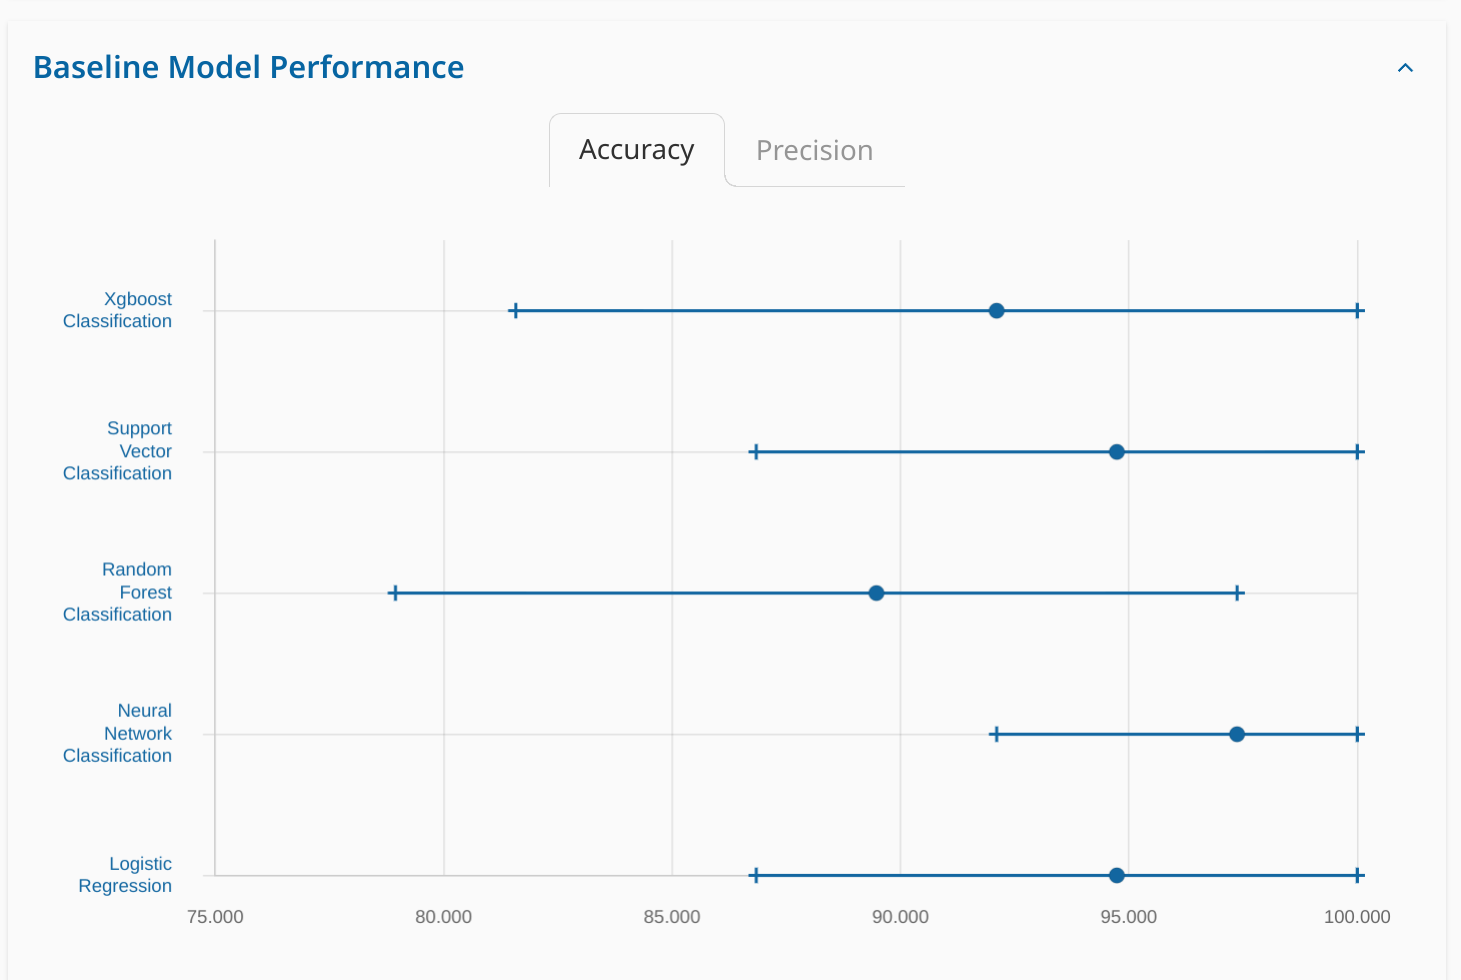
\includegraphics[width=0.7\textwidth,height=\textheight]{../res/screenshot_ucmi_perfs.png}
\caption{performances attendu d'après le UCI ML Repo \cite{IrisWebsite}}
\end{figure}

Ce résultat illustre bien que notre démarche est correcte et que nos 2
modèles sont efficaces, avec un penchant pour la régression logistique
qui semble être plus efficace que Naive Bayes.

\paragraph{2.2.5.2 Résultats obtenus pour la régression logistique
multinomiale}\label{ruxe9sultats-obtenus-pour-la-ruxe9gression-logistique-multinomiale}

Suite à l'apprentissage du modèle multinomiale, on obtien les
performances suivantes:

\begin{Shaded}
\begin{Highlighting}[]
\NormalTok{python3 main.py}

\NormalTok{Results:}

\NormalTok{Found theta (bias are last column and weights are the rest):}
\NormalTok{[[ 0.32626066  0.83466238 {-}1.21626121 {-}0.55348121  0.17005888]}
\NormalTok{ [ 0.20948959 {-}0.28684921  0.15659967 {-}0.18787991  0.11458452]}
\NormalTok{ [{-}0.53575025 {-}0.54781317  1.05966154  0.74136112 {-}0.2846434 ]]}


\NormalTok{Metrics obtained:}
\NormalTok{\{\textquotesingle{}precision\textquotesingle{}: 1.0, \textquotesingle{}recall\textquotesingle{}: 1.0, \textquotesingle{}accuracy\textquotesingle{}: 1.0, \textquotesingle{}f1\_score\textquotesingle{}: 1.0\}}
\end{Highlighting}
\end{Shaded}

On peut être très satisfait de ces résultats. Pour les obtenir, nous
avons fait le choix de ne pas initialiser aléatoirement la matrice
\(\theta\), mais de l'initialiser à zéros. En effet, comme on n'utilise
que \(1000\) itérations et un \texttt{learning\_rate} de \(10^{-4}\),
initialiser le vecteur avec des valeurs comprises par exemple entre 1 et
10 fera que la descente en gradient optimisera moins bien les paramètres
nécessaire (à cause du faible nombre d'itérations), ce qui n'est pas
l'objectif de l'initialisation aléatoire de la matrice \(\theta\).

Afin de reproduire ces résultats, il suffit de décommenter la ligne
\texttt{\#softmax.main()} dans \code{main.py}

Ici, sur la matrice theta, nous avons chaque ligne qui représente les
poids et biais pour chaque label, avec à chaque fois le dernier élément
de la ligne qui est le biais et le reste qui est le poids.

\newpage{}

\subsection{2.3 -- Naive Bayes}\label{naive-bayes-1}

Dans cette section, une implémentation d'un classifieur linéaire
bayesien (naive bayes) a été réalisée.

\subsubsection{2.3.1 -- Extraction des
distributions}\label{extraction-des-distributions}

Dans cette implémentation, étant données que toutes nos features sont
continues, nous avons considéré que \emph{sepal length}, \emph{sepal
width}, \emph{petal length} et \emph{petal width} seront représenté
comme 4 variables aléatoires \(X_0, \cdots, X_3\) suivant 4 lois
normales normales de paramètre \((\mu_k, \sigma_k)\).

C'est à dire: \[
X_k \sim \mathcal{N}( \mu_k, \sigma_k) \qquad \qquad k \in \iitv{0, 3}
\]

Elles peuvent être récupérées à l'aide de la fonction suivante:

\begin{lstlisting}
def get_distrib_parameters(features: DataFrame, labels) -> dict[Any, list[tuple[fl, fl]]]:
\end{lstlisting}

qui va retourner un dict mappant chaque classe à une liste contenant les
paramètres des distributions conditionnelles (normales) des features
pour cette classe.

\subsubsection{2.3.2 -- Prédictions}\label{pruxe9dictions-1}

Deux fonctions de prédictions ont été implémenté,

\begin{enumerate}
\def\labelenumi{\arabic{enumi}.}
\tightlist
\item
  Prennant un sample et prédisant sa classe
\item
  Une deuxième qui prend tous les samples et applique, en parallèle, la
  première fonction à chacun d'eux.
\end{enumerate}

Elles ont les signatures suivantes:

\begin{lstlisting}
    def predict_bayes(x, params_by_class: dict[Any, list[tuple[fl, fl]]]) -> Any:
    def predict_bayes_all(X: DataFrame, params_by_class: dict[Any, list[tuple[fl, fl]]] | None = None) -> list[Any]:
\end{lstlisting}

Comme dit précédemment, pour pouvoir prédire la classe d'un sample, il
faut calculer les probabilité conditionnelle \(P(\mathbf{x}| classe)\)
pour chaque classe \(y\) et sample \(\mathbf{x}\) et prendre la classe
qui maximise cette dernière.

Cela revient à chercher le \(\tilde{y}\) défini en
\href{#naive-bayes}{section 1.2}, développons le calcul qui nous amené à
cette formule:

\[
\tilde{y}  = \text{arg}\max_{y \in \mathcal{Y}}\ P(y|\mathbf{x}) = \text{arg}\max_{y \in \mathcal{Y}}\ \frac{P(\mathbf{x}|y)  P(y)}{P(\mathbf{x})} =  \text{arg}\max_{y \in \mathcal{Y}}\ P(\mathbf{x}| y)P(y)
\]

Or \[ 
P(\mathbf{x}| y) = P(x_1 | y) \prod_{i = 2}^{n}{P(x_i | x_{i-1}, \ldots, x_1, y)}
\] Avec l'hypothèse que les \(\{X_i\}_{i \leq n}\) sont indépendants, on
obtient que:

\[P(x_i | x_{i-1}, \ldots, x_1, y) = P(x_i | y)\]

Donc
\[P(\mathbf{x}|y) = P(x_1 | y) \prod_{k = 2}^{K}{P(x_k | y)} = \prod_{k=1}^K{P(x_k | y)}\]

En conclusion:
\[ \tilde{y} = \text{arg}\max_{y \in \mathcal{Y}} \left[\  P(y) \prod_{k = 1}^K{P(x_k | y)}\  \right] \]
(où \(K\) reste le nombre de features.)

Où au début on cherche à maximiser \(P(y | x)\) car idéalement on
voudrait savoir la probabilité que \(y\) soit le bon label pour
n'importe quel sample \(\mathbf{x}\). Cependant, on aimerait pouvoir
effectuer cette prédictions pour des \(\mathbf{x}\) qui n'appartiennent
pas à notre dataset d'apprentissage, i.e.~on ne doit pas avoir besoin
d'avoir déjà vu exactement ce sample. On a donc besoin d'une
généralisation, c'est ainsi que l'on fini par retomber sur

\[ \tilde{y} = \text{arg}\max_{y \in \mathcal{Y}} \left[\  P(y) \prod_{k = 1}^K{P(x_k | y)}\  \right] \]

qui est ce que calculent les fonctions dont on a donné la signature
ci-dessus.

\subsubsection{2.3.3 -- Résultats}\label{ruxe9sultats-1}

Dans cette section, nous allons simplement reprendre ce qui a été fait
dit dans la \href{#ruxe9sultats}{section 2.2.4} et remontrer les mêmes
tests.

Voici l'output du test \texttt{pytest} pour les rapports de performances
du model bayesien:

\begin{lstlisting}
src/log_reg.py::test_log_reg_f1score 
weights & biases: [0.53452349, 0.36463584, 1.16132476, 1.08204578], 0.45146791  
{ 'accuracy': 1.0, 'f1_score': 1.0, 'precision': 1.0, 'recall': 1.0 }
PASSED

src/naive_bayes.py::test_predict_bayes_f1score_all  
{ 'accuracy': 0.97, 'f1_score': 0.975, 'precision': 0.976, 'recall': 0.974 }
PASSED
\end{lstlisting}

Ce résultat a été obtenu avec une séparation 70/30 de training/test
data.\\
Ces résultats illustrent bien que notre démarche est correcte et que nos
2 modèles sont efficaces, avec un penchant pour la régression logistique
qui semble être plus efficace que Naive Bayes.\\
Cependant, un f1-score de \(> 0.95\) reste excellent.

\newpage{}

\section{3. -- Analyse}\label{analyse}

Pour chaque classe y, on peut tracer les fonctions de distribution de
probabilité pour chaque donnée \(X_k\) sachant la classe y afin
d'analyser la structure des données.

Pour la classe Y=0, on obtient le graphe suivant :

\begin{figure}
\centering
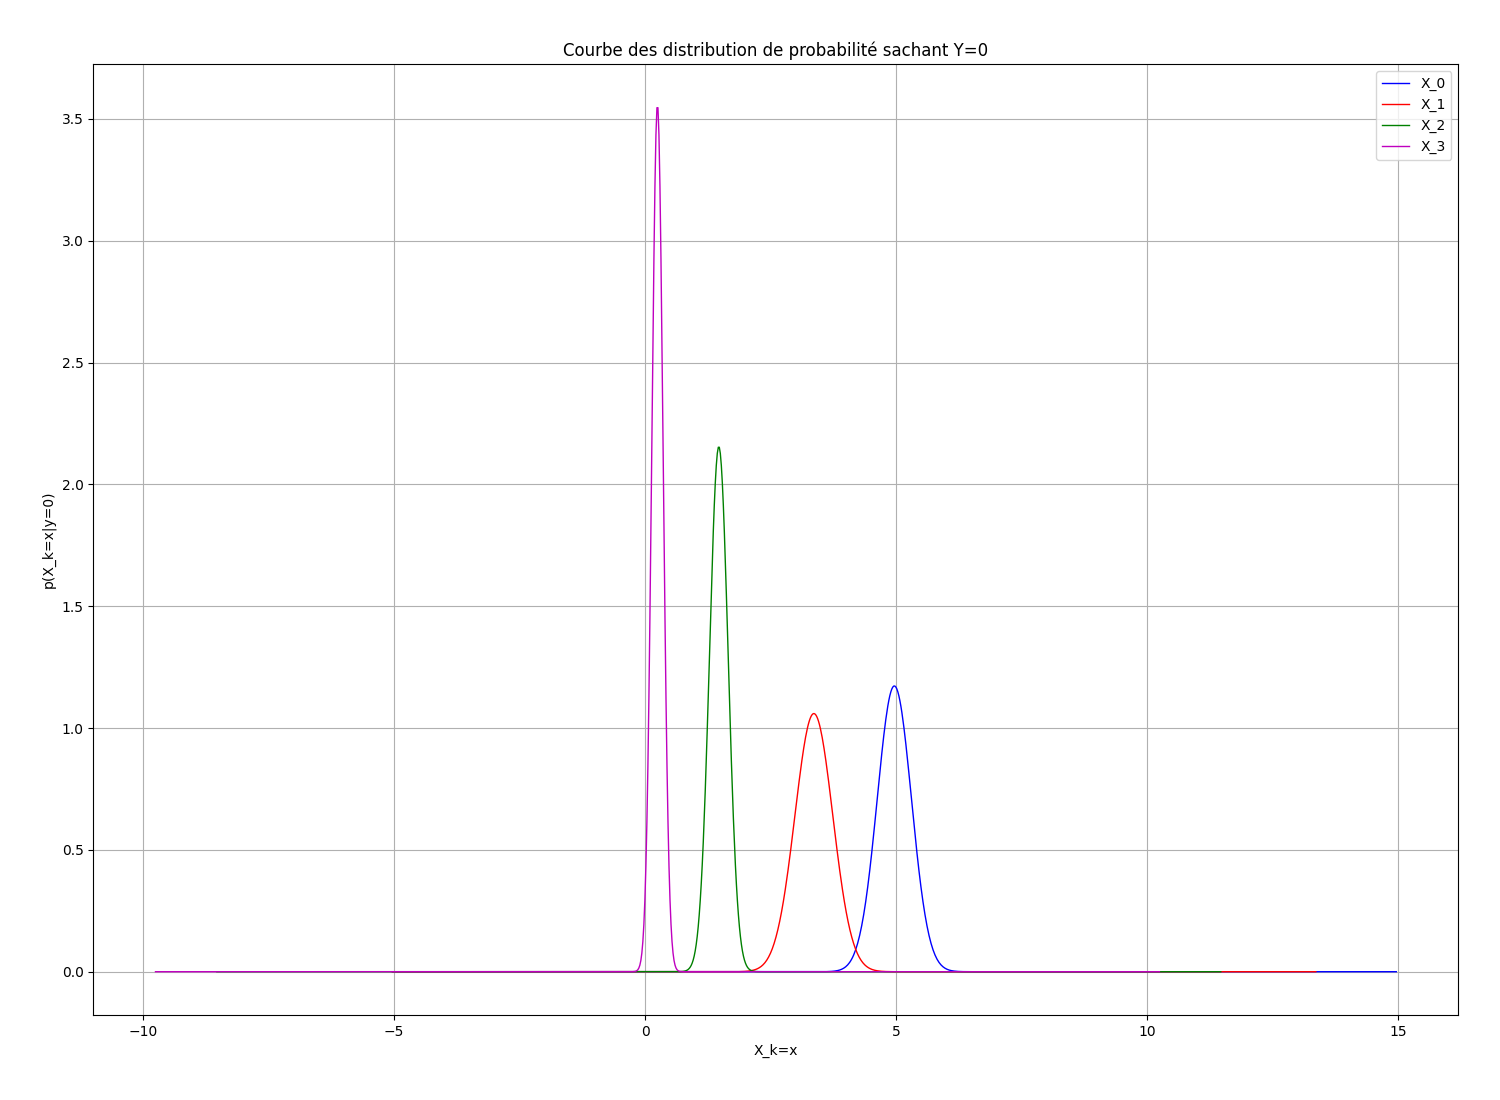
\includegraphics{../src/res/comp_normal_law_Y_0.png}
\caption{graphe des fonctions de distribution sachant Y=0}
\end{figure}

On peut voir tout d'abord que pour cette classe, les pics des courbes
bleue et rouge sont bien inférieurs aux pics des courbes vert et
magenta. Ainsi, on en conclu que les variables \(X_0\) et \(X_1\) ont
moins d'influence dans la prédiction de cette classe. Alors que le pic
de la courbe magenta est bien supérieur aux autres, indiquant que la
variable \(X_3\) a une forte influence sur la prédiction de cette
classe. De plus, on observe que seul les courbent bleu et rouge ont un
chevauchement perceptible mais quand même assez petit, on en conclu que
les variables sont pour cette classe très peu indépendante les unes des
autres.

\newpage{}

Pour la classe Y=1, on obtient le graphe suivant :

\begin{figure}
\centering
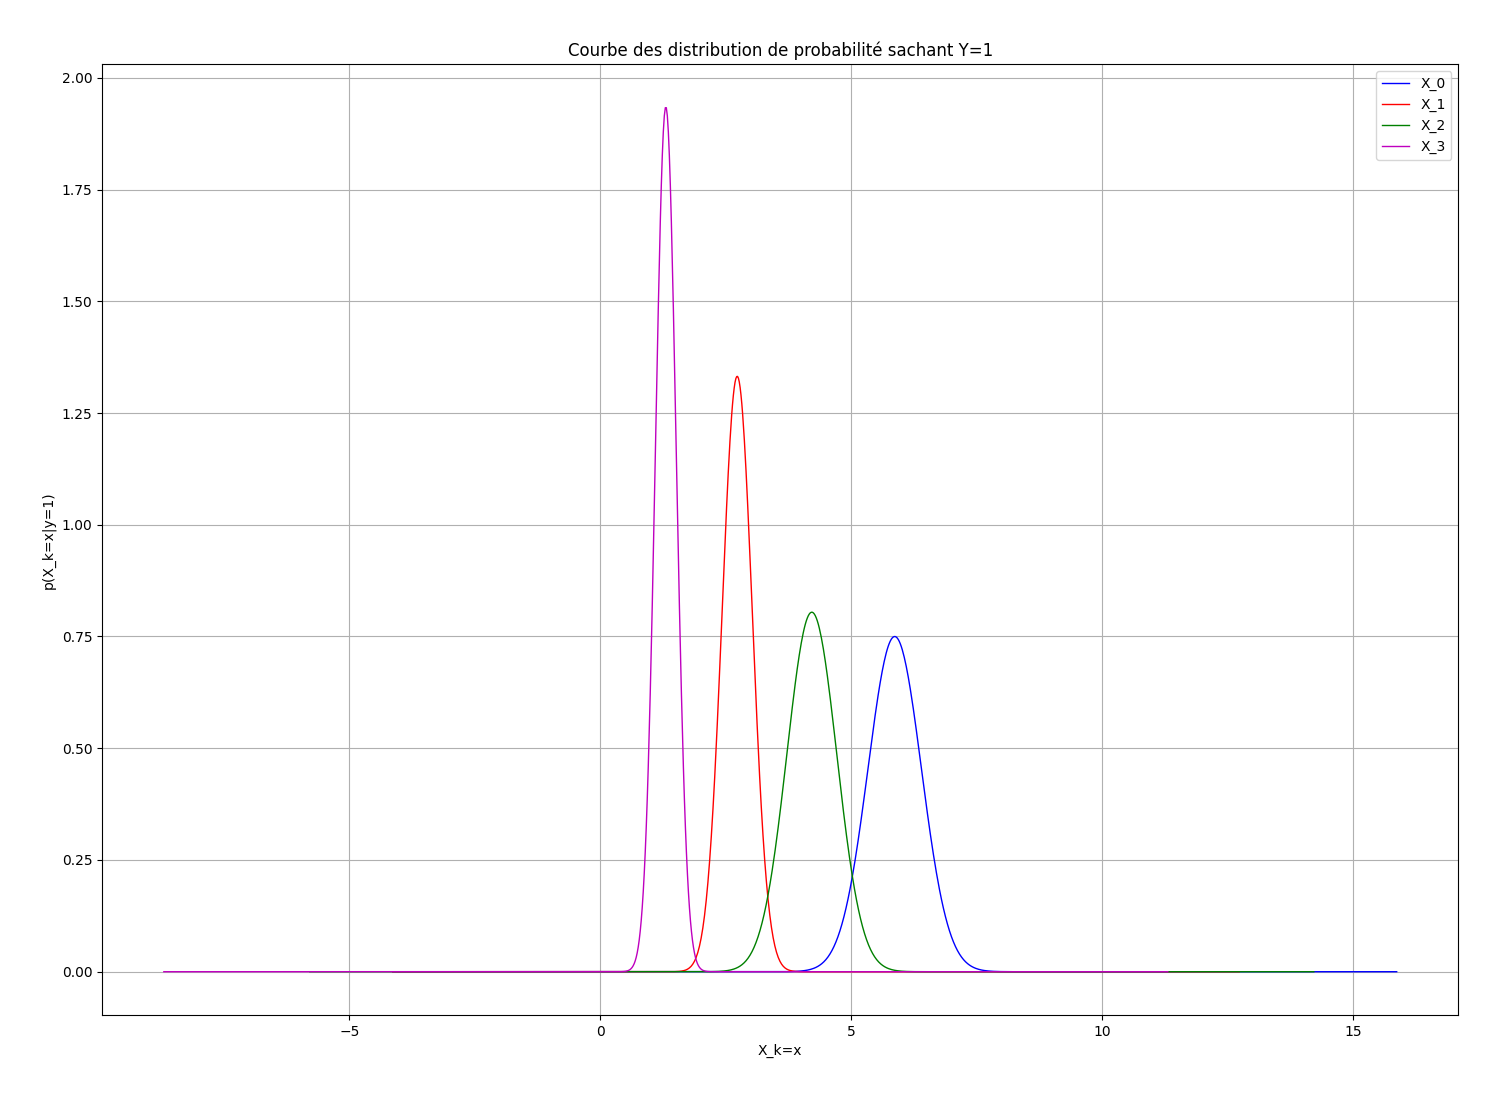
\includegraphics{../src/res/comp_normal_law_Y_1.png}
\caption{graphe des fonctions de distribution sachant Y=1}
\end{figure}

On peut voir tout d'abord que pour cette classe, les pics des courbes
bleus et verte sont bien inférieurs aux pics des courbes rouge et
magenta. Ainsi, on en conclu que les variables \(X_0\) et \(X_2\) ont
moins d'influence dans la prédiction de cette classe. Alors que le pic
de la courbe magenta est bien supérieur aux autres, indiquant que la
variable \(X_3\) a une forte influence sur la prédiction de cette
classe. De plus, on observe que les courbes rouge et magenta ont un
faible chevauchement indiquant une faible interdépence entre \(X_3\) et
\(X_1\) alors que les courbes rouge et verte ainsi que verte et bleue
ont un chevauchement assez élevé montrant une certaine interdépendance
entre les variables \(X_1\) et \(X_2\) ainsi qu'entre les variables
\(X_0\) et \(X_2\).

\newpage{}

Enfin pour la classe Y=2, on obtient le graphe suivant :

\begin{figure}
\centering
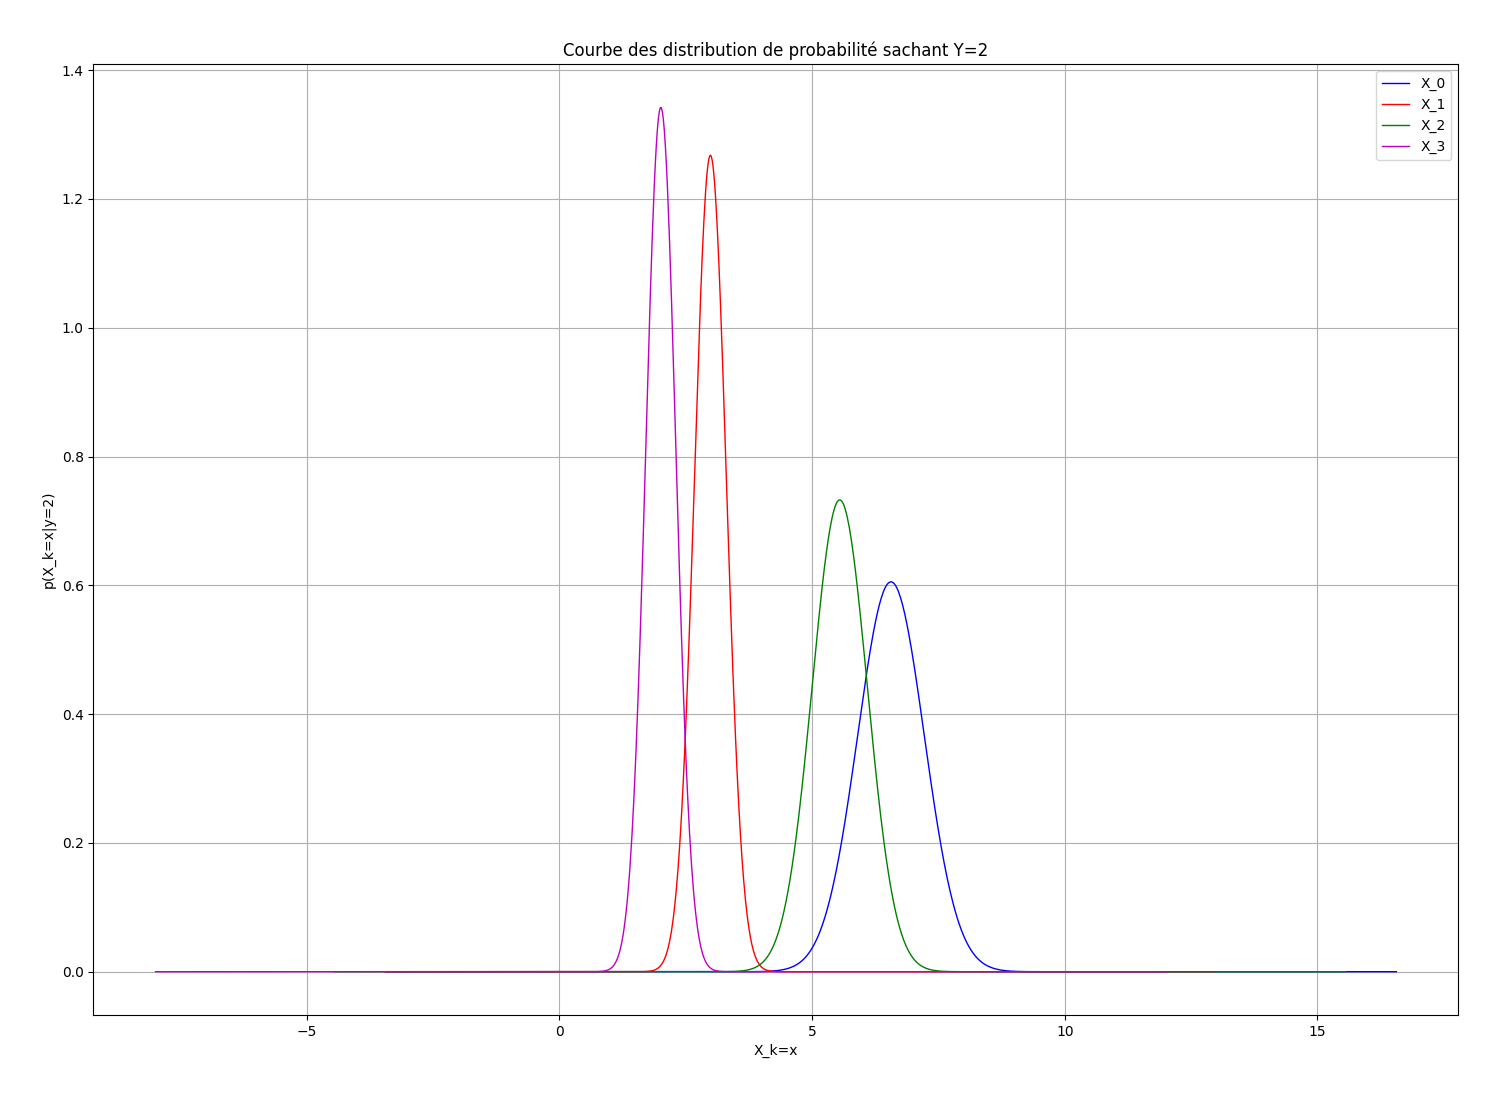
\includegraphics{../src/res/comp_normal_law_Y_2.png}
\caption{graphe des fonctions de distribution sachant Y=2}
\end{figure}

On observe que les pics des courbes rouge et magenta sont presque deux
fois plus grand que ceux des courbes bleue et verte, de plus les courbes
rouge se chevauchent fortement. Ainsi les variables \(X_3\) et \(X_1\)
ont une très forte influence sur cette classe et sont assez
interdépendant alors que les variables \(X_0\) et \(X_2\) ont très peu
d'impacte sur la prédiction de cette classe. Les courbes bleue et verte
se chevauchent aussi énormément montrant aussi une forte interdépendance
entre les variables \(X_0\) et \(X_2\).

Ainsi on peut remarquer que globalement la variable \(X_3\) a une forte
influence sur la classification alors que la variable \(X_0\) a une plus
faible. De plus, les variables indépendantes ne sont pas séparables les
unes des autres.

\subsection{3.1 -- Phénomène de
sur-apprentissage}\label{phuxe9nomuxe8ne-de-sur-apprentissage}

Dans cette partie, nous allons voir les problèmes de sur-apprentissage
du modèle de régression logistique multinomial.

Le phénomène de sur-apprentissage est lorsque le modèle entraîné
s'adapte trop bien aux données d'apprentissage, si bien qu'il s'adapte
au bruit des données d'apprentissage. Cela a pour conséquences de
produire de moins bonnes prédictions pour des données de test. En effet,
le modèle est ``trompé'' par le bruit des données d'apprentissage et
prédira ainsi de mauvais résultats.

Dans l'énoncé, on nous propose d'utiliser un volume de données réduit
afin de montrer le phénomène de sur-apprentissage. Nous étions alors
perplexe et nous nous posions cette simple question: pourquoi utiliser
moins de données pour montrer le phénomène engendré lorsqu'on entraîne
trop un modèle ? À cette question, nous n'avons hélas pas encore trouvé
de réponse qui tranche. En effet, peut-être qu'il faut montrer qu'avec
moins de données, le modèle entraîné peut avoir de bonnes performances
sur les données d'apprentissage, mais pas sur les données de test. Mais
cela ne serait-il pas plutôt un phénomène de sous-apprentissage ? Ou
alors faut-il essayer d'entrainer un maximum notre paramètre \(\theta\)
sur les données d'apprentissage en espérant que notre modèle s'adaptera
trop bien aux données d'apprentissage en donnant de mauvaises
prédictions pour des données de test ? Ou encore doit-on ajouter
beaucoup de bruit dans les données d'apprentissage pour que le modèle
s'entraine sur le bruit des données d'apprentissage et donne de moins
bonnes prédictions pour des données de test ? Bref, ne sachant pas trop
quelle voie explorer, nous avons décidé d'en explorer plusieurs.

Tout d'abord, nous avons testé et entrainé les modèles pour un volume de
données réduit.

Voici 2 graphes montrant les résultats obtenus avec la régression
logistique multinomiale et l'approche naive bayes. Notez que nous avons
tenté de faire une courbe approximant les données obtenues afin de mieux
visualiser ce qu'il se passe. Cette courbe est obtenue, en faisant un
peu de bricolage, par le code suivant:

\begin{Shaded}
\begin{Highlighting}[]
\NormalTok{a, b }\OperatorTok{=}\NormalTok{ np.polyfit(x, log(y), }\DecValTok{1}\NormalTok{)}
\NormalTok{plt.plot(x, a }\OperatorTok{*}\NormalTok{ log(y) }\OperatorTok{+}\NormalTok{ b)}
\end{Highlighting}
\end{Shaded}

Ce qui est une sorte de régression linéaire ``adaptée'' pour une courbe
logarithmique.

\begin{figure}
\centering
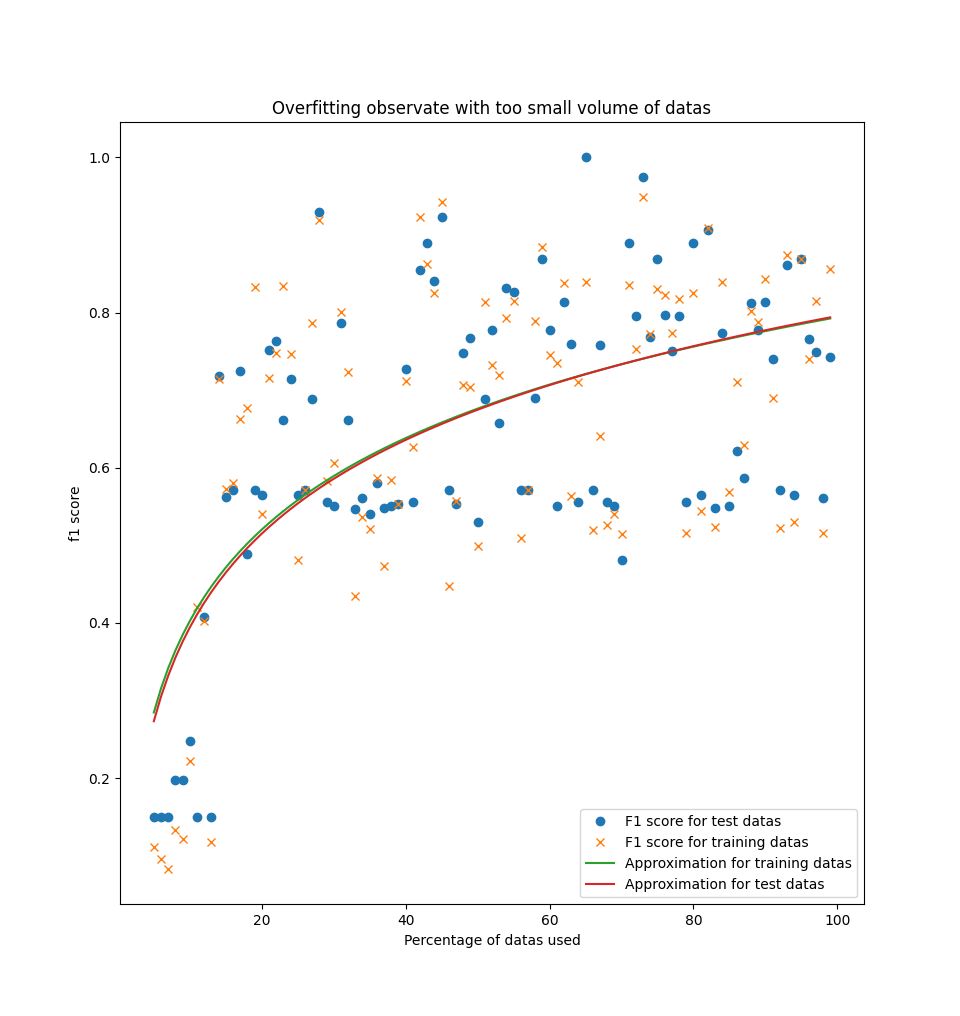
\includegraphics[width=0.67\textwidth,height=\textheight]{../res/overfitting_naive.png}
\caption{Naive bayes}
\end{figure}

\newpage

Sur le graphique donné par Naive Bayes, nous pouvons constater que les
f1 scores varient beaucoup, aussi bien pour les données d'entrainement
que pour les données de test. Cependant, on peut remarquer que pour un
volume faible de données, la courbe verte, correspondant au f1 score
obtenu avec les données d'entrainement, est légèrement au dessus de la
courbe rouge, représentant le f1 score des données de test. Cela
signifie que lorsqu'on n'a pas assez de données d'entrainement, le
modèle entrainé fera ne fera pas de bonnes prédictions sur les données
de test, car celui-ci n'a pas été suffisamment entraîner pour bien
ajuster ses paramètres: ses paramètres sont uniquement ajustés pour les
données d'entrainement.

Cependant, nous pouvons constater que les f1 scores obtenus par Naive
Bayes ne convergent pas\ldots{} C'est pourquoi, afin de montrer les
phénomènes de sur-apprentissage, nous allons utiliser la régression
logistique qui possède des f1 scores convergeant, comme nous pouvons
l'observer sur le graphique.

\begin{figure}
\centering
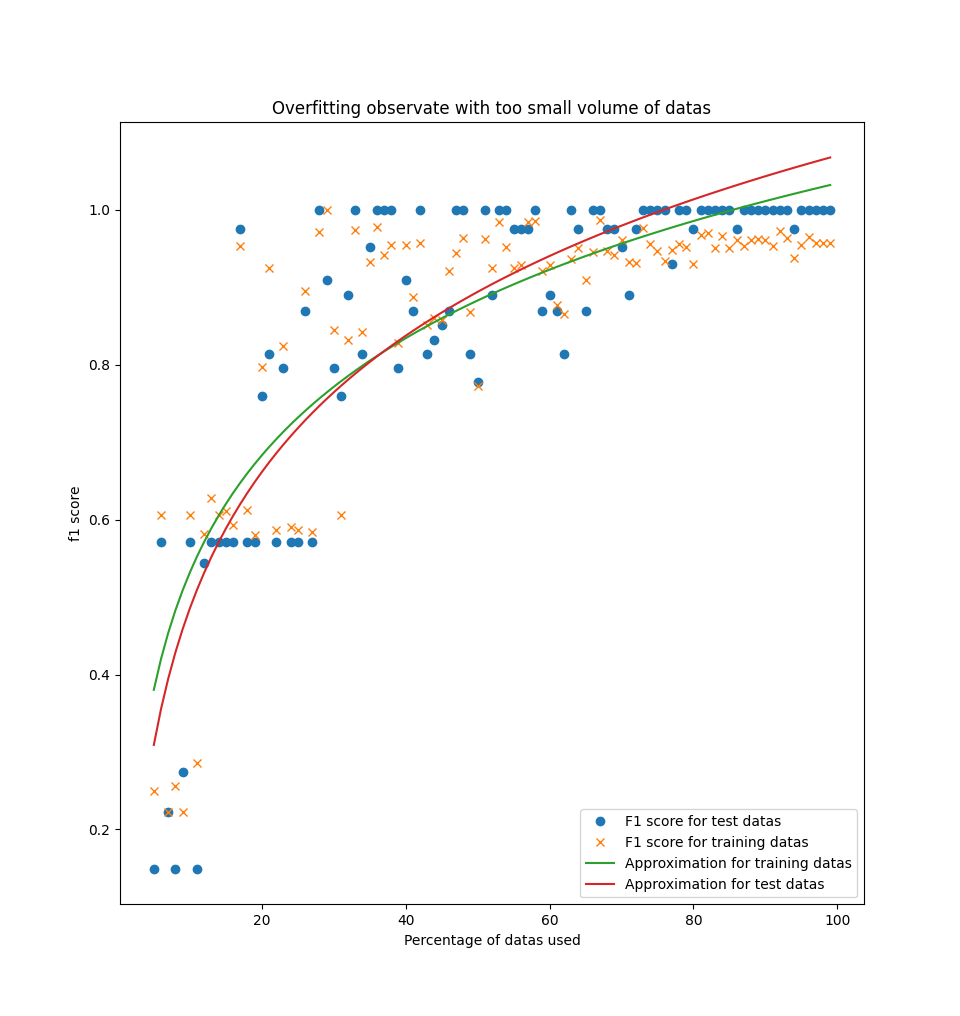
\includegraphics[width=0.67\textwidth,height=\textheight]{../res/overfitting_reg.png}
\caption{Logistic regression}
\end{figure}

Sur le graphique donné par la régression logistique, nous pouvons
observer que les f1 scores sont très variés pour un volume faible de
données, mais que ceux-ci convergent lorsque le volume de données
augmente (On suppose que la même chose se produit avec Naive Bayes, mais
qu'on n'a pas assez de données pour le remarquer\ldots). C'est pour
cette raison que nous allons préférer utiliser la régression logistique
plutôt que Naive Bayes pour montrer les phénomènes de sur-apprentissage.

Nous pouvons également constater que les performances sur les données
d'entrainement sont meilleures que les performances sur les données de
test. Cela montre un ``sur-ajustement'' du modèle sur les données
d'entrainement. En effet, comme le volume de données est faible, les
paramètres de la régression logistique sont bien entraînés pour les
données d'entrainement, mais pas pour les données de test.

Cependant, lorsque le volume de données augmente, on voit que les
paramètres de la régression logistique s'ajustent correctement, et on a
des performances sur les données de test qui deviennent meilleures que
les performances sur les données d'entrainement.

Donc plus on a des données, mieux on pourra ajuster notre modèle. Dans
notre cas, on ne peut pas tester ce que trop de données peuvent faire,
car on n'a hélas pas un stock de données illimité.

Mais nous pouvons nous demander à quel point le bruit peut influencer la
performance de notre modèle.

Afin d'éclaircir ce point, nous allons vous épargner la visualisation du
graphique obtenu par Naive Bayes car celui-ci est très éparse: aucune
donnée ne converge. Mais nous allons vous montrer le graphique obtenu
par la régression logistique.

Tout d'abord, pour ajouter du bruit aux données, nous indiquons un
pourcentage des données qu'on veut bruiter. Ensuite, nous prenons d'une
manière aléatoire le pourcentage donné de données, et pour ces données
sélectionnées, nous attribuons un label aléatoire parmi la liste de
labels initiaux des données. Cela entraine forcément qu'une donnée qu'on
voulait bruiter a repris le même label qu'elle avait, et n'est donc pas
bruité. Donc le bruitage est approximatif.

Voici le graphique obtenu pour la régression logistique:

\begin{figure}
\centering
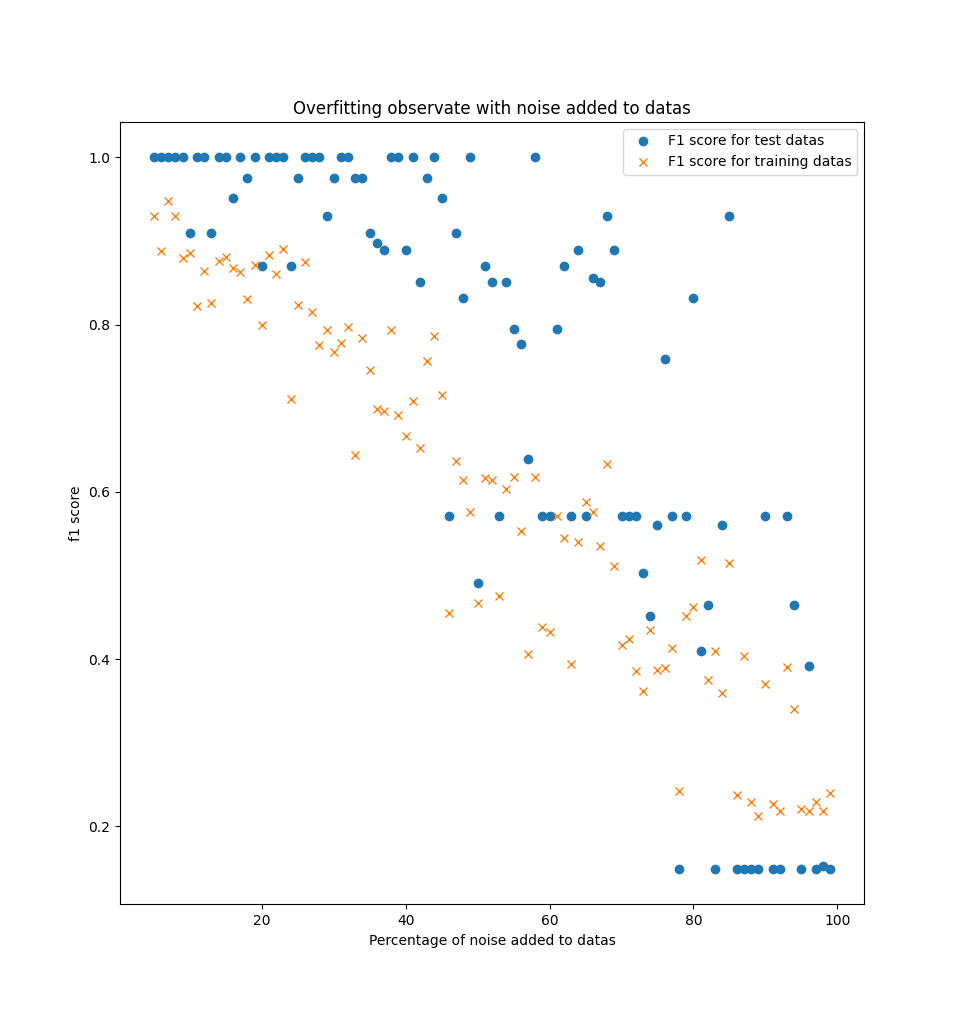
\includegraphics{../res/overfitting_reg_2.png}
\caption{Logistic regression: noise added}
\end{figure}

Nous pouvons constater que pour des données pas très bruitées, le modèle
possède de bonnes performances. Mais plus le bruit introduit dans les
données augmente, plus on obtient des résultats éparpillés et
décroissant dans l'ensemble. Enfin, on peut observer pour 80 à 100\% des
données bruitées que le modèle possède de très mauvaises performances
sur les données de test, qui sont moins bonnes que les performances
obtenues sur les données d'entrainement. Cela est causé par le bruit
introduit dans les données: il y a suffisamment de bruit dans les
données pour que le modèle soit entrainné au bruit des données
d'apprentissage, ce qui cause de mauvaises performances sur des données
de test.

Donc trop de bruit dans les données d'apprentissage d'un modèle peut
rendre un modèle avec de mauvaises performances, car trop entrainé au
bruit des données d'apprentissages.

Enfin, nous avons tenté de faire varier le nombre d'itérations lors de
la descente en gradient de la régression logistique et ajouté du bruit
aux données pour que les paramètres de la régression logistique soient
perturbés par le bruit des données. Nous avons mis 50\% de bruit dans
les données d'apprentissage, ce qui nous a donné le graphe suivant:

\begin{figure}
\centering
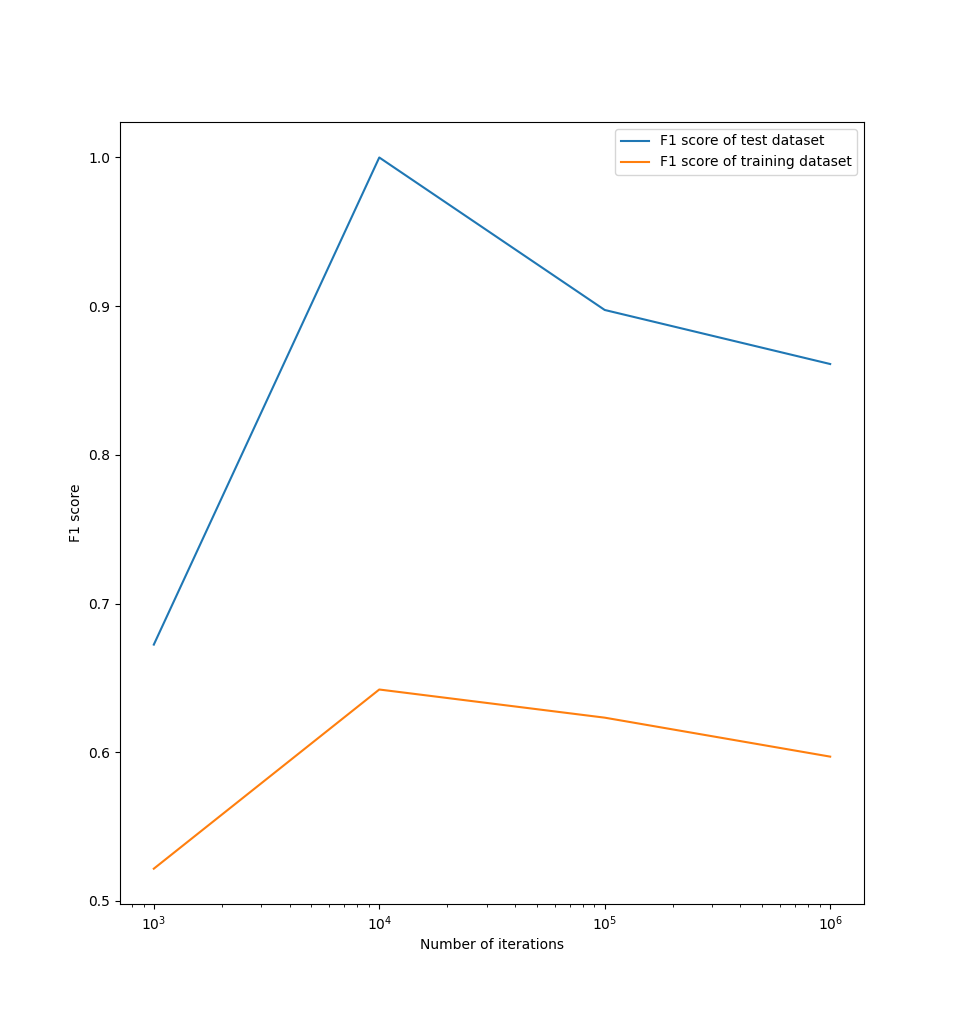
\includegraphics{../res/overfitting_test.png}
\caption{Logistic regression: varying number of iterations}
\end{figure}

Les résultats nous plaisent car ils montrent que pour un faible nombre
d'itérations, les performances du modèle sont bonnes, mais moins bonnes
que pour un nombre moyen d'itérations, et pour un nombre trop grand
d'itérations, les performances du modèle sont moins bonnes.

Cela signifie que si la descente en gradient est trop précise, on aura
un modèle bien entrainé pour les données d'apprentissage, mais pas pour
les données de test, car la performance du modèle sur les données de
test diminue lorsqu'on a un nombre d'itérations élevé, tandis que la
performance du modèle reste à peu près constante pour les données
d'entrainement.

Ainsi, il faut également ajuster la précision de la descente en gradient
afin d'obtenir non pas les paramètres optimaux pour les données
d'apprentissage, mais pour obtenir des paramètres à la fois généraux et
précis, permettant de donner des performances optimales sur des données
de test.

Nous pouvons conclure que le sur-apprentissage ou sur-ajustement peut
causer des problèmes dans les performances d'un modèle de
classification, comme la régression logistique, car le modèle peut soit
s'entrainer trop au bruit des données d'apprentissages, entrainant de
mauvais résultats de test, soit ne pas avoir suffisamment de données
d'apprentissage pour bien ajuster ses paramètres, soit trop s'entrainer
aux données d'apprentissage, ce qui entraine une baisse de performance
sur les données de tests, car le modèle est également entrainé au bruit
des données d'apprentissage.

Enfin, il faut toujours s'assurer que le modèle donne les meilleures
performances possibles sur les données de test, car les performances sur
les données de test comptent plus que les performances sur les données
d'apprentissage\ldots{}

\subsubsection{3.1.1 -- Fonctions et
signatures}\label{fonctions-et-signatures}

Pour bruiter les données, une fonction a été créée dans
\code{overfitting.py}. Cette fonction possède la signature suivante:

\begin{lstlisting}
    def add_noise_to_data(labels: np.ndarray, percentage: int) -> np.ndarray:
\end{lstlisting}

Elle prend des données aléatoirement et les bruite en réatribuant le
label correspondant aux caractéristiques. On peut avoir le label qui est
défini d'une manière aléatoire à sa valeur initiale.

Pour prendre seulement un pourçentage des données, une autre fonction a
été créée dans \code{overfitting.py}. Cette fonction possède la
signature suivante:

\begin{lstlisting}
    def get_percentage_of_data(feat: np.ndarray, labels: np.ndarray, percentage: int) -> np.ndarray:
\end{lstlisting}

Cette fonction prend un pourcentage des données qui ont été, au
préalable, ``mélangées'' aléatoirement.

Les graphiques ont été obtenus grâce aux autres fonctions définies dans
\code{overfitting.py}. On peut les exécuter en décommentant les lignes
suivantes de la toute fin de \code{overfitting.py} et en décommentant la
ligne \texttt{overfitting.main()} de main:

\begin{Shaded}
\begin{Highlighting}[]
\CommentTok{\#overfitting\_naive\_bayes(FEAT, LABELS, FEAT\_test, LABELS\_test)}
\CommentTok{\#overfitting\_log\_reg(FEAT, LABELS, FEAT\_test, LABELS\_test)}
\CommentTok{\#overfitting(FEAT, LABELS, FEAT\_test, LABELS\_test)}
\end{Highlighting}
\end{Shaded}

Le code peut cependant prendre du temps à l'exécution: il prennait
environ 2 minutes à tourner sur la machine d'un des étudiants.

\newpage{}

\section{4 -- Comparaisons}\label{comparaisons}

\subsection{4.1 - Vraisemblance et classification des
échantillons}\label{vraisemblance-et-classification-des-uxe9chantillons}

Une fois que les paramètres des classes sont obtenus en supposant
l'indépendance des variables, on échantillone de nouvelles données afin
de comparer les résultats obtenus avec les données d'origine.

L'échantillonage est fait dans le fichier \texttt{sampling.py}.

On fait 50 échantillons pour chaque classe, à partir des paramètres des
distributions obtenus dans la section précédente.

On obtient les résultats suivants (la moyenne et l'écart-type sont
donnés pour chaque classe et chaque variable):

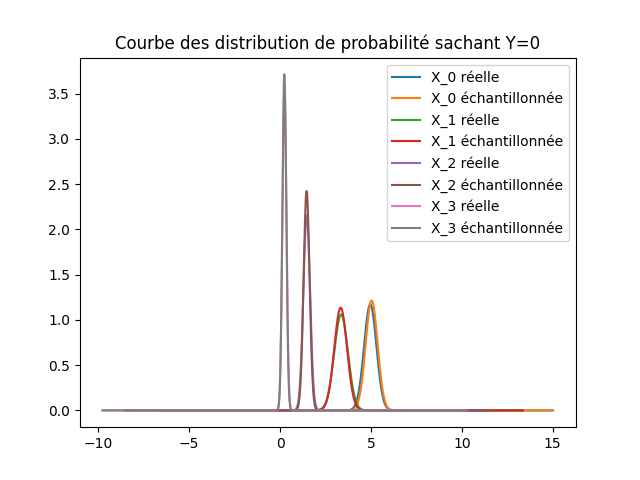
\includegraphics{../res/sample_compare_Y_0.png}
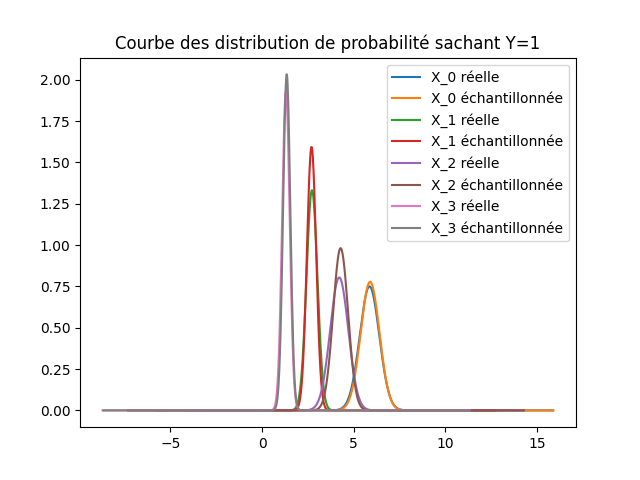
\includegraphics{../res/sample_compare_Y_1.png}
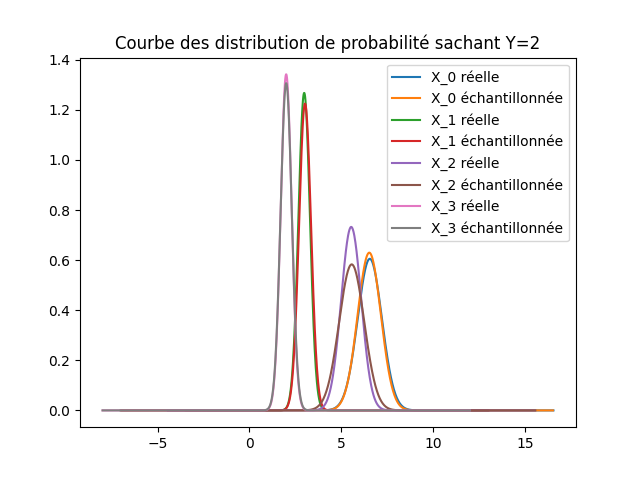
\includegraphics{../res/sample_compare_Y_2.png}

\begin{itemize}
\tightlist
\item
  Pour la classe 0:

  \begin{itemize}
  \tightlist
  \item
    Mean:

    \begin{itemize}
    \tightlist
    \item
      réelle: 4.964516, 3.3612902, 1.467742, 0.2451613
    \item
      échantillon: 5.04191904, 3.33580458, 1.46340112, 0.23831319
    \end{itemize}
  \item
    Ecart-type:

    \begin{itemize}
    \tightlist
    \item
      réel: 0.34014544, 0.37654343, 0.18508933, 0.112067565
    \item
      échantillon: 0.32847194, 0.35161457, 0.16439592, 0.10696828
    \end{itemize}
  \end{itemize}
\item
  Pour la classe 1:

  \begin{itemize}
  \tightlist
  \item
    Mean:

    \begin{itemize}
    \tightlist
    \item
      réelle: 5.862162, 2.7243242, 4.2108107, 1.3027027
    \item
      échantillon: 5.89406553, 2.70037139, 4.28611674, 1.3473438
    \end{itemize}
  \item
    Ecart-type:

    \begin{itemize}
    \tightlist
    \item
      réel: 0.531952, 0.29944894, 0.49597478, 0.20613708
    \item
      échantillon: 0.51264886, 0.25024787, 0.40643571, 0.19599569
    \end{itemize}
  \end{itemize}
\item
  Pour la classe 2:

  \begin{itemize}
  \tightlist
  \item
    Mean:

    \begin{itemize}
    \tightlist
    \item
      réelle: 6.5594597, 2.9864864, 5.545946, 2.0054054
    \item
      échantillon: 6.52999239, 3.0324595, 5.57314614 2.00670609
    \end{itemize}
  \item
    Ecart-type:

    \begin{itemize}
    \tightlist
    \item
      réel: 0.65889615, 0.31460926, 0.54446435, 0.29715872
    \item
      échantillon: 0.63336966, 0.32560175, 0.68418903, 0.30524206
    \end{itemize}
  \end{itemize}
\end{itemize}

Les nombres et les graphiques montrent que les échantillons sont très
proches des données réelles, donc on a bien la vraisemblance.

\subsection{4.2 - Comparaison avec
SKLearn}\label{comparaison-avec-sklearn}

\subsubsection{4.2.1 - Naïve Bayes}\label{nauxefve-bayes}

Notre implémentation de Naïve Bayes a été comparée avec celle de SKLearn
dans le fichier \texttt{sampling.py}, avec un split des données
échantillonnées en 70\% training et 30\% test.

On obtient les résultats suivants:

Notre Naive Bayes

\begin{itemize}
\item
  Precision: 0.9761904761904763
\item
  Recall: 0.9743589743589745
\item
  Accuracy: 0.9777777777777777
\item
  F1\_score: 0.9752738654147106
\end{itemize}

Sklearn Naive Bayes

\begin{itemize}
\item
  precision: 0.9761904761904763
\item
  recall: 0.9743589743589745
\item
  accuracy: 0.9777777777777777
\item
  f1\_score: 0.9752738654147106
\end{itemize}

\subsubsection{4.2.2 - Régression
Logistique}\label{ruxe9gression-logistique-2}

Notre implémentation de Régression Logistique a été comparée avec celle
de SKLearn dans le fichier \texttt{sampling.py}, avec un split des
données échantillonnées en 70\% training et 30\% test.

Pour SKLearn, le modèle utilisé est
\texttt{lr\ =\ LogisticRegression(multi\_class="multinomial")}, car on a
3 classes et donc il nous faut un modèle multinomial.
\cite{sklearnLogReg}

Notre Logistic Regression

\begin{itemize}
\item
  Precision: 0.8505050505050505
\item
  Recall: 0.8461538461538461
\item
  Accuracy: 0.8666666666666667
\item
  F1\_score: 0.848323868840447
\end{itemize}

Sklearn Logistic Regression

\begin{itemize}
\item
  Precision: 0.9761904761904763
\item
  Recall: 0.9743589743589745
\item
  Accuracy: 0.9777777777777777
\item
  F1\_score: 0.9752738654147106
\end{itemize}

\subsection{4.3 - Conclusion sur les
comparaisons}\label{conclusion-sur-les-comparaisons}

On a vu qu'on avait la vraisemblance, puisque les échantillons sont très
proches des données réelles, comme le montrent les graphiques.

En ce qui concerne SKLearn, on peut voir que les métriques pour Naïve
Bayes sont identiques car les 2 implémentations sont simplement une
application du théorème de Bayes, donc on espère avoir les mêmes
résultats.

Pour le logistic regression, SKLearn fournit de meilleurs métriques car
il est certainement plus optimisé que notre implémentation.

Malgré cela, notre implémentation donne quand même des très bons
résultats, avec chaque métrique tournant autour de 85\%.

On a donc aussi la classification.

On peut donc conclure que les deux implémentations arrivent à bien
classifier les données IRIS.

\newpage{}

\section{5 -- Contributions}\label{contributions}

\subsection{Noah Munz}\label{noah-munz}

\begin{itemize}
\tightlist
\item
  Mise en place du repos github
\item
  Mise en place du code
\item
  Mise en place du dataset
\item
  Implémentation de \code{naive\_bayes.py} et de \code{log\_reg.py}
\item
  Auteur des sections:

  \begin{itemize}
  \tightlist
  \item
    1
  \item
    2.0
  \item
    2.1
  \item
    2.2.3
  \item
    2.2.4.1
  \item
    2.2.5.1
  \item
    2.3
  \end{itemize}
\end{itemize}

\subsection{Gregory Sedykh}\label{gregory-sedykh}

\begin{itemize}
\tightlist
\item
  Implémentation de \code{sampling.py}
\item
  Auteur de la section 4
\end{itemize}

\subsection{Noah Petershmitt}\label{noah-petershmitt}

\begin{itemize}
\tightlist
\item
  Implémentation de \code{plot\_util.py} ?
\item
  Auteur de la section 3 (jusqu'à 3.1)
\end{itemize}

\subsection{Léandre Catogni}\label{luxe9andre-catogni}

\begin{itemize}
\tightlist
\item
  Implémentation de \code{metrics.py}
\end{itemize}

\subsection{Michel Donnet}\label{michel-donnet}

\begin{itemize}
\tightlist
\item
  Implémentation de \code{softmax.py}, de \code{gradient\_descent.py} et
  de \code{overfitting.py}
\item
  Auteur des sections

  \begin{itemize}
  \tightlist
  \item
    2.2.1
  \item
    2.2.2
  \item
    2.2.4.2
  \item
    2.2.5.2
  \item
    3.1
  \end{itemize}
\end{itemize}

\newpage

\printbibliography[heading=bibintoc, title={Références}]

\end{document}
